\documentclass[dvipdfmx,a4j,10pt]{jsarticle}
\usepackage{amsthm}%定理環境
\usepackage{newtxtext,newtxmath}%times font setting
\usepackage{amsmath,amsfonts}%数式font setting
\usepackage{mathrsfs}%花文字
\usepackage{pxrubrica}%ルビ
%\usepackage{lmodern}%font setting
\usepackage{mathtools}%数式の相互参照部分にのみ式番号をふる
\mathtoolsset{showonlyrefs,showmanualtags}
\usepackage{empheq}%方程式
\usepackage{physics}%物理系
\usepackage{bm}%vector
\usepackage{mleftright}%カッコ
\usepackage{framed}%フレーム
\usepackage{color}
\usepackage{tikz}
\usepackage{booktabs}%表の上線\toprule中線下線\bottomrule
\usepackage{url}%参考文献とかでurlをかくとき
%\usepackage[dvipdfmx]{hyperref}%ハイパーリンク
%\usepackage{comment}
\usepackage{tcolorbox}
\tcbuselibrary{theorems,skins}%数式を「デコ」る
\usepackage{tikz}
\usetikzlibrary{patterns}
\usetikzlibrary{cd}%矢印の図
\usetikzlibrary{decorations,decorations.pathreplacing}%数式を「デコ」る
\pgfdeclarepatternformonly{south west lines}{\pgfqpoint{-0pt}{-0pt}}{\pgfqpoint{3pt}{3pt}}{\pgfqpoint{3pt}{3pt}}{
	\pgfsetlinewidth{0.4pt}
	\pgfpathmoveto{\pgfqpoint{0pt}{0pt}}
	\pgfpathlineto{\pgfqpoint{3pt}{3pt}}
	\pgfpathmoveto{\pgfqpoint{2.8pt}{-.2pt}}
	\pgfpathlineto{\pgfqpoint{3.2pt}{.2pt}}
	\pgfpathmoveto{\pgfqpoint{-.2pt}{2.8pt}}
	\pgfpathlineto{\pgfqpoint{.2pt}{3.2pt}}
	\pgfusepath{stroke}
}
\usepackage{bbm}
\usepackage{ascmac}
\usepackage{lscape}
\usepackage{caption}
\usepackage{boites}
\usepackage{here}

%\setcounter{secnumdepth}{4}%セクションの深さレベル

%\makeatletter%subsubsubsection定義
%    \newcommand{\subsubsubsection}{\@startsection{paragraph}{4}{\z@}%
%        {1.0\Cvs \@plus.5\Cdp \@minus.2\Cdp}%
%        {.1\Cvs \@plus.3\Cdp}%
%        {\reset@font\sffamily\normalsize}
%    }
%\makeatother

%physicsでrotもcurlで使う
\newcommand{\rot}{\curl}

\newtheoremstyle{mystyle1}% Name
    {}% Space above
    {}% Space below
    {\normalfont}% Body font
    {}% Indent amount
    {\bfseries\sffamily}% Theorem head font
    {\hspace{0.5em}}% Punctuation after theorem head
    { }% Space after theorem head, ‘ ‘, or \newline
    {\thmname{#1}\thmnumber{#2}\thmnote{(#3)\\}}% Theorem head spec (can be left empty, meaning `normal')
\theoremstyle{mystyle1}
\newtheorem{dfn}{定義}[section]
\newtheorem{thm}[dfn]{定理}
\newtheorem{axi}[dfn]{公理}
\newtheorem{cor}[dfn]{系}
\newtheorem{prop}[dfn]{命題}
\newtheorem{lem}[dfn]{補題}
\newtheorem{exs}[dfn]{例題}
\newtheorem{note}[dfn]{注意}
\newtheorem{ex}[dfn]{例}

\newtheoremstyle{mystyle2}% Name
    {}% Space above
    {}% Space below
    {\normalfont}% Body font
    {}% Indent amount
    {\bfseries\sffamily}% Theorem head font
    {\hspace{0.5em}}% Punctuation after theorem head
    { }% Space after theorem head, ‘ ‘, or \newline
    {\thmname{#1}\thmnote{(#3)\\}}% Theorem head spec (can be left empty, meaning `normal')
\theoremstyle{mystyle2}
\newtheorem{dfn*}{定義}
\newtheorem{thm*}{定理}
\newtheorem{prop*}{命題}
\newtheorem{example}{例}
\newtheorem{qes}{問題}
\newtheorem{note*}{注意}
\newtheorem{ans}{解答}
\newtheorem{lem*}{補題}

%proofの後ろに黒四角をつける
\makeatletter
\renewenvironment{proof}[1][\proofname]{\par
  \pushQED{\qed}%
  \normalfont
  \topsep6\p@\@plus6\p@ \trivlist
  \item[\hskip\labelsep{\bfseries\sffamily #1}]\ignorespaces
}{%
  \popQED\endtrivlist\@endpefalse
}
\renewcommand\proofname{証明}
\renewcommand{\qedsymbol}{\ensuremath{\blacksquare}}
\makeatother

%ansの後ろに黒四角をつける
\makeatletter
\renewenvironment{ans}[1][解答]{\par
  \pushQED{\qed}%
  \normalfont
  \topsep6\p@\@plus6\p@ \trivlist
  \item[\hskip\labelsep{\bfseries\sffamily #1}]\ignorespaces
}{%
  \popQED\endtrivlist\@endpefalse
}
\renewcommand{\labelenumi}{\ensuremath{\blacksquare}}
\makeatother

%方程式番号にセクション番号を入れる(subsectionまで)
\makeatletter
\@addtoreset{equation}{section}
\def\theequation{\thesubsection.\arabic{equation}}% renewcommand でもOK
\makeatother

\makeatletter
\renewcommand{\thefigure}{% 図番号の付け方
\thesection.\arabic{figure}}
\@addtoreset{figure}{section}
\makeatother

%\renewcommand{\thepart}{\arabic{part}}
%\renewcommand{\thenote}{}
%\renewcommand{\thelem}{}

%\makeatletter
%\@addtoreset{section}{part}
%\makeatother

%\makeatletter
%\def\blfootnote{\xdef\@thefnmark{}\@footnotetext}
%\makeatother

%\setcounter{tocdepth}{1}%目次をsectionまでの表示にする

\newcommand{\blueunderline}[3][pos=0.5]{
    \tcboxmath[
        enhanced,
        frame hidden, % 枠を消す
        interior hidden, % 背景を消す
        size=minimal, % 余白を消す
        overlay={
                \draw[
                    blue,
                    decorate
                ] ([yshift=-4pt]frame.south west) -- ([yshift=-4pt]frame.south east)
                node[#1,scale=0.8,below] {#3};
            }
    ]{#2}
}

\newenvironment{textleftbrace}
{$\left\{
	\begin{tabular}{l}
}
{	\end{tabular}
	\right.
	$\vspace{0.25\baselineskip}
}

\renewcommand{\labelenumi}{(\arabic{enumi})}%enumerateのデフォルトを(1)などにする
\newcommand{\defLeftrightarrow}{\overset{\text{def}}{\iff}}
\newcommand*{\defeq}{\stackrel{\text{def}}{=}}
\DeclareMathOperator{\Ob}{Ob}
\DeclareMathOperator{\Ar}{Ar}
\DeclareMathOperator{\dom}{dom}
\DeclareMathOperator{\cod}{cod}
\DeclareMathOperator{\Hom}{Hom}
\newcommand{\Sets}{\mathbf{Sets}}
\newcommand{\Set}{\mathbf{Set}}
\newcommand{\Mon}{\mathbf{Mon}}
\newcommand{\Cat}{\mathbf{Cat}}
\newcommand{\Graph}{\mathbf{Graph}}
\newcommand{\Pos}{\mathbf{Pos}}
\newcommand{\tabitem}{~~\llap{\textbullet}~~}

\def\startpoint#1{
    {\hfill\rlap{{$\overline{\tt{#1}\ \downarrow\ }$}}}\vspace{-1.5\baselineskip}
}

\title{情報数学I}
\author{担当:三好}
%\date{}%コメントアウトした状態だと今日の日付が入る
\begin{document}
\maketitle
教科書:Category Theory, Second Edition, Steve Awodey, (Oxford University Press, 2010)

\url{http://www.andrew.cmu.edu/course/80-413-713/notes/}

\begin{note*}
	章番号を教科書に合わせているので番号が前後している場合があります.
\end{note*}

\tableofcontents%目次

\newpage

\section{圏論}

\paragraph{集合論}

\begin{itemize}
	\item 現れるのは集合のみ
	\item メンバーシップ関係$\in$
\end{itemize}

$a,b$を集合とする.$a,b$について関係$a\in b$が成り立つ.\\
$\Rightarrow$ $b$は$a\in b$が成り立つすべての要素$a$の集まり\\
$\Rightarrow$集合という概念の本質(外延性)

\begin{example}
	2つの集合$b,b'$が等しい($b=b'$)とは,$\in$により定義される.
	\[
		\forall x(x\in b\to x\in b')\land \forall x'(x'\in b'\to x'\in b)
	\]
	($b$と$b'$とは$\in$では区別できないとき等しい)
\end{example}

\paragraph{関係$R$と関数$f$}

\begin{dfn*}[関係]

	$X,Y$:集合
	\[
		(a,b)\in R\subset X\times Y=\{(x,y)|x\in X\land y\in Y\}
	\]
	のとき$a$と$b$は$R$という関係にあると考える.(関係は集合!)
\end{dfn*}

\begin{example}
	実数$\mathbb{R}$上の$=$や$\leq$も$\mathbb{R}$上の二項関係.
\end{example}

\begin{dfn*}[関数(写像)]
	関数$f\subset X\times Y$が関数($=$写像\footnote{本講義では関数と写像を同じ意味として扱う})であるとは,次の2つの条件を満たすことをいう.
	\begin{enumerate}
		\item 一意性:$(x,y),(x',y')\in f\Rightarrow y=y'$
		\item 全域性:$\forall x\in X,\exists y \in Y$($(x,y)\in f$)
	\end{enumerate}
	このとき,$f:X\to Y$,もしくは$X\xrightarrow{f} Y$とかく.$(a,b)\in f$のとき$f(a)=b$とかく.
\end{dfn*}

\begin{itemize}
	\item 関数も関係であり,よって集合である.
	\item 関数の同値性は集合の同値性で決まる(外延的同値).
	      $f,f':X\to Y$
	      \[
		      \forall a\in X(f(a)=f'(a))\defLeftrightarrow f=f'
	      \]
	      これの左側を集合論的に書くと$\forall a\in X ((a,f(a))=(a,f'(a)))$.
	\item 同じ入力に同じ出力を返す関数は同じ関数(関数名やアルゴリズムは見ていない)
\end{itemize}

\paragraph{関数の合成}

集合:$A,B,C$,関数$f:A\to B,g:B\to C$とする.

\begin{dfn*}[合成関数]
	$f$と$g$の合成関数$g\circ f:A\to C$は,各$a\in A$について
	\[
		(g\circ f)(a)\defeq g(f(a))
	\]
	により定義される(外延性より一意的).
\end{dfn*}

\begin{prop*}[結合律]
	$f:A\to B, g:B\to C, h:C\to D$に対して
	\[
		h\circ (g\circ f)=(h\circ g)\circ f
	\]
\end{prop*}
\begin{proof}
	合成の定義による.
\end{proof}

\begin{dfn*}[恒等関数]
	各集合$A$について恒等関数$\mathbbm{1}_A:A\to A$は,$\forall a\in A$について$\mathbbm{1}_A(a)\defeq a$により定義される.
\end{dfn*}

\begin{prop*}[恒等射律]
	$f:A\to B$のとき
	\[
		\mathbbm{1}_A\circ f=f,f\circ \mathbbm{1}_B=f
	\]
	となる.
\end{prop*}

\begin{proof}
	合成の定義と恒等関数の定義により示せる.
\end{proof}

このように関数では定義から結合律や恒等写律が証明できる.

\begin{itemize}
	\item 圏論とは,\textbf{関数の抽象代数}という側面をもつ(Awodey)
	\item 圏論とは,\textbf{普遍性(非常にリッチな極限)}を取り扱う理論.
	      これらを扱うために
	      \begin{itemize}
		      \item limit(極限)/ colimit(余極限)
		      \item adunction(随伴)
		      \item representability(説明可能性)(Universal Mapping Property)
	      \end{itemize}
\end{itemize}

\paragraph{圏論にまつわる歴史}

集合から集合への関数から,構造付き集合から構造付き集合への構造を保つ関数(=準同型)を考えたいというモチベーションが生まれた.

\begin{table}[htb]
	\begin{tabular}{llll}
		1940s & 代数トポロジー                       & 1945 & Eilenberg-MacLane                       \\
		      & \tabitem ホモロジー代数              &      & "General theory of natural equivalence" \\
		      & \tabitem 抽象代数                    &      &                                         \\
		1950s & A.Grothendieck Tohoku Paper(1957)    & 1954 & N.Yoneda 米田の補題                     \\
		      & \tabitem 代数幾何                    &      & "On the Homology Theory of Modules"     \\
		      & \tabitem アーベル群                  & 1958 & D.Kan "Adjoint factors" 随伴の発見      \\
		1960s & F.W.Lawvere et al.                   &      &                                         \\
		      & 圏論と論理のつながり                 &      &                                         \\
		      & 圏を対象とする研究グループの出現     &      &                                         \\
		1970s & (冬の時代)                         &      &                                         \\
		      & 他分野への応用                       &      &                                         \\
		      & \tabitem コンピュータ科学            &      &                                         \\
		      & \tabitem 論理学                      &      &                                         \\
		      & \tabitem 認知科学                    &      &                                         \\
		      & \tabitem 哲学                        &      &                                         \\
		1980s & コンピュータ科学と論理学との結びつき &      &                                         \\
		      & さらにこれらと圏論との結びつき       &      &                                         \\
	\end{tabular}
\end{table}

圏論の応用:表現論,佐藤超関数,Motives(代数幾何,数論)

\paragraph{様々な圏}

\begin{itemize}
	\item ファイバー圏(1960 -)Benabou Street
	\item enriched cats(1960 - )Street Kelly Day ...
	\item 2-cats bicat(1960s -)Street Kelly Day Benabou ...
	\item Strict higher dim cats(1960 - )Ehresmann
	\item コヒーレンスを持つ弱高次元圏の定義の発見(基本的に$(\omega,\omega)$-圏,$(m,m)$-圏)\\
	      1995 Baez-Dalam Batanin \\
	      2000 Leinster Cheng
	\item 結び目定理とモノイダル圏の結びつき(late 1980s -)\\
	      Yetter, Joyal, Street
	\item gausi cat, $(\infty,1)$-catsの整備\\
	      A. Joyal(late 1990s -)\\
	      J. Lurie(2000s -)
	\item 応用圏論(2010 -)F.Y.Gaimard proofret線形型\\
	      モノイダル圏と線形論理の対応(1990s)(線形論理はCS的に重要)\\
	      圏論的量子論(2000s)
\end{itemize}

\newpage

\setcounter{subsection}{2}

\subsection{記号や言葉の定義}

\begin{itemize}
	\item 対象と射:
	      \begin{itemize}
		      \item 対象(object):$A,B,C,\ldots$
		      \item 射(arrow):$f,g,h,\ldots$
	      \end{itemize}
	\item 圏$\mathcal{C}$において
	      \begin{itemize}
		      \item $\Ob(\mathcal{C})$:対象すべての集まり
		      \item $\Ar(\mathcal{C})$:射すべての集まり
	      \end{itemize}
	\item 各射$f\in \Ar(\mathcal{C})$について,ドメインとよばれる対象$\dom(f)$とコドメインとよばれる対象$\cod(f)$が\underline{一意的に}割り当てられている.一意的というのは,関数で表せる,ということ:
	      \begin{itemize}
		      \item $\dom :\Ar(\mathcal{C})\to \Ob(\mathcal{C})$
		      \item $\cod :\Ar(\mathcal{C})\to \Ob(\mathcal{C})$
	      \end{itemize}
	      $\dom(f)=A$かつ$\cod(f)=B$のとき,$f:A\to B$と書く(関数の記法を借用.$A,B$の中身の構造については何も考えていない.)
	      \begin{note*}
		      グラフ理論では,対象をnode,射をedge,ドメインをsource,コドメインをtargetとよぶ.
	      \end{note*}
	      ドメインが$A$,コドメインが$B$の射全体の集まりを特に$\mathcal{C}(A,B)$もしくは$\Hom_{\mathcal{C}}(A,B)$と書き\footnote{準同型homomorphicからきている.},ホムセット(homset)とよぶ.\\
	      これにより,合成の定義がしやすくなるだけでなく,圏論を展開していく上(representabilityを扱うとき)で重要な役割を果たす.
	\item 合成付きグラフ:
	      \begin{center}
		      \vspace{-1zh}
		      \begin{tikzcd}[row sep=0.5ex]
			      (-)\circ (-):\mathcal{C}(B,C)\times \mathcal{C}(A,B) \arrow[d,phantom,"\rotatebox{90}{$\in$}",shift left=5.3ex] \arrow[r]& \mathcal{C}(A,C) \arrow[d,phantom,"\rotatebox{90}{$\in$}"]\\
			      \qquad\qquad\quad (g,f) \arrow[r,mapsto] &
			      \tcboxmath[
				      enhanced,
				      frame hidden, % 枠を消す
				      interior hidden, % 背景を消す
				      size=minimal, % 余白を消す
				      overlay={
						      \draw[
							      blue,
							      decorate
						      ] ([yshift=-4pt]frame.south west) -- ([yshift=-4pt]frame.south east)
						      node[pos=1.5,scale=0.8,below] {関数合成の記号を借用};
					      }
			      ]{g\circ f}
		      \end{tikzcd}
	      \end{center}
	      \vspace{0.5\baselineskip}
	      合成が一意的であるので関数として表せる.結合律を満たすことを定義として要請する.
	\item 圏:任意の$A\in\Ob(\mathcal{C})$について,$\mathbbm{1}_A:A\to A$で恒等射律をみたすものの存在を要請する(一意性は示せる.$\mathbbm{1}_A=\mathbbm{1}_A\circ\mathbbm{1}_{A'}=\mathbbm{1}_{A'}$).
\end{itemize}
\footnote{圏の定義ここ読んでもなんかパッとしないから教科書も見た方がいいかも.}
関数で成り立っていた代数構造を定義として要請しているのが圏である.

\subsection{圏の例}

\begin{example}[Set]
	対象を集合とみなし,射を関数(=写像)とみなせばよい.
\end{example}

\begin{example}[有限な例]
	\ \vspace{-1zh}
	\begin{enumerate}
		\item
		      \begin{tikzcd}
			      0 \arrow[out=30,in=330,loop,"\mathbbm{1}_0"]
		      \end{tikzcd}
		\item
		      \begin{tikzcd}
			      0 \arrow[out=150,in=210,loop,"\mathbbm{1}_0"'] \arrow[r,"f"] & 1 \arrow[out=30,in=330,loop,"\mathbbm{1}_1"]
		      \end{tikzcd}
		\item
		      \begin{tikzcd}
			      0 \arrow[out=150,in=210,loop,"\mathbbm{1}_0"'] \arrow[r,"f_0"] \arrow[rd,"f_1\circ f_0"'] & 1 \arrow[d,"f_1"] \arrow[out=75,in=15,loop,"\mathbbm{1}_1"] \\
			      & 2 \arrow[out=30,in=330,loop,"\mathbbm{1}_2"]
		      \end{tikzcd}
		      \setcounter{enumi}{-1}
		\item 空圏
	\end{enumerate}
\end{example}

\begin{example}[自由生成]
	任意の適当なグラフに必要なものを付け加えて圏を生成することができる.
	\begin{center}
		\begin{tikzcd}
			& \cdot \arrow[rd] & \\
			\cdot \arrow[ru] & & \cdot
		\end{tikzcd}
		$\Longrightarrow$
		\begin{tikzcd}
			& \cdot \arrow[out=125,in=55,loop] \arrow[rd] & \\
			\cdot \arrow[out=150,in=210,loop] \arrow[ru] \arrow[rr] & & \cdot \arrow[out=30,in=330,loop]
		\end{tikzcd}
	\end{center}
\end{example}

\begin{example}[Partially Ordered Set, poset $(X,\leq)$]
	\ \vspace{-\baselineskip}
	\begin{enumerate}
		\item $\forall x\in X\,(x\leq x)$
		\item $\forall x,y,z\in X,\,x\leq y\land y\leq z\Rightarrow x\leq z$
		\item $\forall x,y\in X,\, x\leq y\land y\leq x\Rightarrow x=y$
		\item $\forall x,y\in X,\, x\leq y \lor y\leq x$
	\end{enumerate}
	(1)(2)を満たすのがpreorder(前順序),(1)(2)(3)を満たすのがpartial order(半順序),(1)(2)(3)(4)を満たすのがlinear order(全順序).$X$を対象の集合,$\leq$を射とみなすと(1)(2)により圏になる.

	\begin{figure}[H]
		\begin{minipage}{0.45\hsize}
			\begin{center}
				\begin{tikzcd}
					& \cdot \arrow[out=120,in=60,loop] & \\
					\cdot \arrow[out=210,in=150,loop] \arrow[ru] & & \cdot \arrow[out=30,in=330,loop] \arrow[lu] \\
					& \cdot \arrow[out=240,in=300,loop] \arrow[lu] \arrow[uu] \arrow[ru] &
				\end{tikzcd}
			\end{center}
			\caption*{partial order, not linear order}
		\end{minipage}
		\begin{minipage}{0.45\hsize}
			\begin{center}
				\begin{tikzcd}
					& \cdot \arrow[out=120,in=60,loop] & \\
					\cdot \arrow[out=210,in=150,loop] \arrow[ru] \arrow[rr,bend left=15,crossing over] & & \cdot \arrow[out=30,in=330,loop] \arrow[lu] \arrow[ll,bend left=15,crossing over] \\
					& \cdot \arrow[out=240,in=300,loop] \arrow[lu] \arrow[uu] \arrow[ru] &
				\end{tikzcd}
			\end{center}
			\caption*{preorder, not partial order}
		\end{minipage}
	\end{figure}

	(以下は圏の定義を満たすことの確認)
	\begin{enumerate}\renewcommand{\labelenumi}{(\alph{enumi})}
		\item 任意のドメインとコドメインの間の射は高々1つ.
		\item 任意の対象について(1)と(a)より恒等射が存在する.
		\item 射の合成は(2)と(a)より一意的に存在する.
	\end{enumerate}

	以上をふまえて圏\textbf{Pos}を考えよう

	\subparagraph{圏$\mathbf{Pos}$}
	\begin{itemize}
		\item 対象:partial order set
		\item 射:順序構造を保存する関数(=単調関数).partial order setの準同型と考えることもできる.
		      \footnote{$f:(X,\leq_X)\to (Y,\leq_Y)$($f:X\to Y,\, x,y\in X$)$x\leq_X y\,\Rightarrow\,f(x)\leq_Y f(y)$}
	\end{itemize}
\end{example}

\begin{example}[Rel]
	圏は対象だけでは決まらないという例.
	\begin{itemize}
		\item 対象:集合(\textbf{Set}と同じ)
		\item 射:関係(\textbf{Set}と異なる)\\
		      (関係$f\subset A\times B$のドメインは$A$,コドメインは$B$,関数ではないが$f:A\to B$とも書く.)
		\item 恒等射:$\mathbbm{1}_A=\{(a,a)\in A\times A| a\in A\}\subset A\times A$
		\item 合成:
		      関係$R\subset A\times B$および$S\subset B\times C$について,関係の合成$S\circ R$は次のように定義される:
		      \[
			      (a,c)\in S\circ R \defLeftrightarrow \exists b\in B((a,b)\in R\land (b,c)\in S)
		      \]
		      (外延性により各組について定義すれば定まる.)
	\end{itemize}
	これらが結合律と恒等射律を満たすことは容易に示せる.よってこれらは圏$\mathbf{Rel}$を定義する.
\end{example}

集合の圏や群の圏などとよくいうが,射も決まらないと圏も決まらないということに注意.

\begin{dfn*}[concrete categories]
	インフォーマルには対象が集合+構造,射が構造を保つ(準同型とよばれる)関数であるような圏のこと.\textbf{Pos}や\textbf{Set}などが例.
\end{dfn*}

射が関数でない圏はconcrete categoriesとは呼ばないことが多い(理由は後述).

\begin{example}[モノイド(monoid)(単位的半群)]
	1つの構造を圏とみるものの例.モノイドの集合+構造である$M=\langle \hat{M},(\textrm{-})\cdot(\textrm{-}),u\rangle$\footnote{$(\textrm{-})\cdot (\textrm{-})$は中値演算子のこと}とは以下のようなものである.

	\begin{itemize}
		\item $\hat{M}$:the underlying set(底集合).$M$とも書く.
		\item $u$:unit(単位元).$e$とも書く.
		\item $\begin{cases}
				      (-)\cdot(-):\hat{M}\times\hat{M}\to\hat{M} \\
				      u\in\hat{M}
			      \end{cases}$\,\textrm{s.t.}\,
		      $\begin{cases}
				      \textrm{(1)}\,\forall x,y,z\in\hat{M},\, x\cdot(y\cdot z)=(x\cdot y)\cdot z \\
				      \textrm{(2)}\,\forall x\in\hat{M},\, u\cdot x=x=x\cdot u
			      \end{cases}$\footnote{(1)のみのものはsemigroupとよばれる.}
	\end{itemize}
	(2)を満たす要素は存在すれば一意的である\\
	($\because$$u,u'$がどちらも単位元のとき$u=u\cdot u'=u'$となる.左の等号は$u'$,右の等号は$u$についての(2)を用いた.)

		\subparagraph{モノイド準同型(monoid homomorphism)}\

	$M=\langle \hat{M},(\textrm{-})\cdot_M(\textrm{-}),u_M\rangle$,$N=\langle \hat{N},(\textrm{-})\cdot_N(\textrm{-}),u_N\rangle$はモノイド.
		関数$f:\hat{M}\to\hat{N}$が次の性質を満たすとき,モノイド準同型と呼ばれる:
		\begin{enumerate}\renewcommand{\labelenumi}{(\alph{enumi})}
			\setcounter{enumi}{1}
			\item $f(u_M)=u_N$
			\item $f(x\cdot_M y)=f(x)\cdot_N f(y)$
		\end{enumerate}
		このとき,任意のあるモノイド構造$M$は,対象が1つの圏$\hat{M}$とみなすことができる.
	\begin{itemize}
		\item $\Ob(\hat{M})=\{*\}$(一点集合)とおく.
		\item $\Ar(\hat{M})=\hat{M}$とおく.
		\item 任意の$x\in \hat{M}$について$x:*\to *$とおく.
		\item モノイド演算$(\textrm{-})\cdot(\textrm{-})$を射の合成とみなす.
		\item $u\in\hat{M}$を$*$の恒等射$\mathbbm{1}_{*}$とする.
	\end{itemize}
	\begin{center}
		\begin{tikzcd}
			* \arrow[out=30,in=330,loop,"x"] \arrow[out=120,in=60,loop,"u"] \arrow[out=210,in=150,loop,"y\cdot x"] \arrow[out=300,in=240,loop,"y"]
		\end{tikzcd}
	\end{center}
	このとき,モノイドの条件(1)より結合律が成り立ち,条件(2)より恒等射律が成り立つ.
	この対応は逆も成り立つので対象の違いをのぞき同一視できる.

	\subparagraph{モノイドと関手}\
	モノイドを圏とみなしたとき,モノイド準同型は関手とみなせる.
	\begin{center}
		\quad\qquad
		\begin{tikzcd}
			* \arrow[out=30,in=330,loop,"x"] \arrow[out=120,in=60,loop,"u_M"] \arrow[out=210,in=150,loop,"y\cdot_Mx"] \arrow[out=300,in=240,loop,"y"]
		\end{tikzcd}
		\qquad
		\begin{tikzcd}
			f(*) \arrow[out=20,in=340,loop,"f(x)"] \arrow[out=120,in=60,loop,"f(u_M)=u_N"] \arrow[out=200,in=160,loop,"f(y\cdot_Mx)=f(y)\cdot_Nf(x)"] \arrow[out=300,in=240,loop,"f(y)"]
		\end{tikzcd}\\
		\begin{tikzcd}
			f:\hat{M} \arrow[r] & [25ex] \hat{N}
		\end{tikzcd}
	\end{center}

	\subparagraph{圏$\Mon$}
	\begin{itemize}
		\item 対象:モノイド
		\item 射:モノイド準同型
	\end{itemize}
	とする圏.

\end{example}

%pos monoid 集合に構造が入ったもの それらがなす圏としてposを考えた
%順序構造の準同型とみなすことができる
%圏はObとAr集まりの上の構造だと見ることができる

圏も「構造をもつ集合」とみなすと,「構造を保つ関数」を考えることができる.

\begin{dfn*}[関手]
	$\mathcal{C},\mathcal{D}$を圏とする.$F:\mathcal{C}\to\mathcal{D}$を関数$F_0:\Ob(\mathcal{C})\to\Ob(\mathcal{D})$,$F_1:\Ar(\mathcal{C})\to\Ar(\mathcal{D})$の組$(F_0,F_1)$とする(添字は明らかな場合は省略する).$F$が次の3つの条件を満たすとき,関手(functor)と呼ぶ.
	\begin{enumerate}\renewcommand{\labelenumi}{(\alph{enumi})}
		\item $F(f:A\to B)=F(f):F(A)\to F(B)$\\
		      ($F_0(\dom(f))=\dom(F_1(f)),\,F_0(\cod(f))=\cod(F_1(f))$.すなわち$\dom,\cod$の構造を保つ)
		\item $A\in\Ob(\mathcal{C})$のとき,$F(\mathbbm{1}_A:A\to A)=\mathbbm{1}_{F(A)}:F(A)\to F(A)$\\
		      ($F_1(\mathbbm{1}_A)=\mathbbm{1}_{F_0(A)}$.すなわち恒等射の構造を保つ)
		\item $f:A\to B,\, g:B\to C$のとき$F(g\circ f)=F(g)\circ F(f)$\\
		      (すなわち合成の構造を保つ)
	\end{enumerate}
	なお,この3つの性質(a)(b)(c)を関手性(functoriality)と呼ぶ((a)は自明として略されることもある).
\end{dfn*}

\begin{itemize}
	\item 関手の合成は$F_0,F_1$の合成より定義できる.よって結合律をみたす.
	\item 恒等関手は$F_0,F_1$が恒等関数であると定義できる.よって恒等射律をみたす.
\end{itemize}
よって,圏を対象とし,関手を射とみれば,圏と関手からなる圏を考えることができる.

\begin{example}[\textbf{Pos}]
	Posの準同型は,Posを圏とみたときの関手になっている.実際$f:(X,\leq_X)\to (Y,\leq_Y)$として
	\begin{enumerate}\renewcommand{\labelenumi}{(\alph{enumi})}
		\item $f((x,y))=(f(x),f(y))$より順序保存.
		\item $f((x,x))=(f(x),f(x))$.反射律と高々1つより,
		\item $f((y,z)\circ (x,y))=f(x,z)=(f(x),f(z))=(f(y),f(z))\circ (f(x),f(y))$
	\end{enumerate}
	となって関手性をみたすことが確認できる.
\end{example}

しかし正確にはもう少し注意深く考えなければならない(次節).

圏の定義において
\begin{itemize}
	\item $\Ob(\mathcal{C})$と$\Ar(\mathcal{C})$がどちらも大きな集合であるとき圏$\mathcal{C}$を大きな圏(large category)と呼び,$\Ob(\mathcal{C})$と$\Ar(\mathcal{C})$がどちらも小さな集合であるとき圏$\mathcal{C}$を小さな圏(small category)と呼ぶ.
	\item 大きな圏すべてを対象とし,関手を射とする圏を\textbf{CAT}と書き,小さな圏すべてを対象とし,関手を射とする圏を\textbf{Cat}と書く.
	\item 圏$\mathcal{C}$の任意の対象$A,B$について,$\mathcal{C}(A,B)$が小さな集合であるとき$\mathcal{C}$を局所小圏(locally small category)とよぶ.
\end{itemize}

\begin{example}[\textbf{Set};locally smallだがnot smallな例]
	$\Ob(\textbf{Set})$と$\Ar(\textbf{Set})$は共に大きな集合であるが,任意の(小さな)集合$A,B$について$\textbf{Set}(A,B)$は(小さな)集合である($\because$関数の定義より).
\end{example}

\setcounter{subsection}{7}

\subsection{集まりの大きさの問題}

圏の定義のときに「集合」と書かずに「集まり」と書いたのには理由がある.

すべての集合の集まり$U$は集合か?という問を考えたとき,答えはNoである.もし集合であったなら$U\in U$が成り立つはずだが,このような集合の存在は矛盾を引き起こす(Russell Paradox).しかし圏論では集合ではない(大きな)集まりを多用する.
\begin{example}[\textbf{Set}]
	$\Ob(\textbf{Set})$は集合ではない.$\Ar(\textbf{Set})$も集合でない.
\end{example}
構造をもつ集合とその準同型からなる圏も同様である(\textbf{Pos},\textbf{Grp},\textbf{Rng},etc).この問題をなんとかしたい.

\vspace{0.5\baselineskip}

\subparagraph{解決法その1(Grothendiech)}

より大きな集まりを扱える集合論で圏論を展開する.

NBG集合論:ZFC集合論の拡大であり,集合すべての集まりのような大きな集まりが組み込まれており,クラス(class)と呼ばれる
(たいていはNBG集合論を直接使うのではなくZFCを用いて大きな集まりが現れるときだけクラスという名称を借用することが多い).

しかし一般にはすべてのクラスを集めたときに再び同様の問題が起こる.

Grothendiechの解決法(SGs4):
(強)到達不能基数(inaccessible cardined)の存在を仮定する.そうすれば,集合を対するクラスのようなより大きな集まりの階層を構成することができる.$\blacksquare$

\vspace{0.5\baselineskip}

\subparagraph{解決法その2(MacLane)}

基数に言及するのではなくユニバースと呼ばれる特殊な集合の存在を仮定する.
\begin{dfn*}[ユニバース]
	空でない集合$\mathcal{U}$がユニバースであるとは,次の4条件を満たすことである:
	\begin{enumerate}
		\item $x\in y\in \mathcal{U}$ならば$x\in \mathcal{U}$($\in$の左方に閉じている)
		\item $x,y\in \mathcal{U}$ならば$\{x,y\}\in\mathcal{U}$(対の構成について閉じている)
		\item $x\in\mathcal{U}$ならば$\mathcal{P}\defeq\{y|y\subset x\}\in\mathcal{U}$(冪集合について閉じている)
		\item $I\in \mathcal{U}, i\in I,x_i\in I$ならば$\bigcup_{i\in I}x_i\defeq\{y|\exists i\in I(y\in x_i)\}\in \mathcal{U}$($I\in\mathcal{U}$の添字の和集合について閉じている)
	\end{enumerate}
\end{dfn*}
$\mathcal{U}$がユニバースならば次が成り立つ(証明略):
\begin{enumerate}\setcounter{enumi}{4}
	\item $\phi\in\mathcal{U}$
	\item $x\in\mathcal{U}$ならば$\{x\}\in\mathcal{U}$
	\item $x\in\mathcal{U}$ならば$\bigcup_{y\in x}y\in\mathcal{U}$
	\item $x,y\in\mathcal{U}$ならば$x\times y\in\mathcal{U}$
	\item $I\in\mathcal{U},i\in I,x_i\in\mathcal{U}$ならば$\coprod_{i\in I}x_i\in\mathcal{U},\prod_{i\in I}x_i\in\mathcal{U}$
\end{enumerate}
すなわち,$\mathcal{U}$は通常の集合の操作について閉じている.そこで$\mathcal{U}$の要素を新たに<集合>と呼ぶにしても通常の数学が展開できる.そこで,ZFCに次の公理を加える:
\begin{center}
	\textbf{公理:}$\mathbb{N}\in\mathcal{U}$をみたすユニバース$\mathcal{U}$が存在する
\end{center}
すると$\mathcal{U}$は集合でもあるので$\mathcal{U}$に対する集合的操作を新たに定義しなおす必要はない.また,$\mathcal{U}$を要素とする別のユニバース$\mathcal{U}$の存在も公理から導かれるため,ユニバースの階層も方法1と同様に構成される.$\blacksquare$
\vspace{0.5\baselineskip}

これらの2つの方法のどちらを採用しても,理論の展開に大きな違いはない.
方法1の集合,あるいは方法2の$\mathcal{U}$の集合を小さな集合(small set),方法1のクラスあるいは方法2の$\mathcal{U}$の要素を大きな集合(large set)と呼び,これらを区別することのみが圏論にとって重要である.

この講義では関数,関係などの再定義が不要であるため,方法2を採用することにする.(圏論的モデル論など集合論と圏論の両方が関わる分野ではもう少し慎重になる必要がある.)

% 4/26 ここから ----------

\startpoint{4/26(第3回)}

\setcounter{subsection}{4}

\subsection{同型性}

\begin{dfn*}[同型射(isomorphism)/ 逆射(inverse)]
	圏$\mathcal{C}$の射$f:A\to B$が\textbf{同型射(isomorphism)}であるとは,次の条件をみたす射$g:B\to A$が存在することをいう:
	\[
		\begin{split}
			g\circ f&=\mathbbm{1}_A\\
			f\circ g&=\mathbbm{1}_B
		\end{split}
	\]
	$g$を$f$の\textbf{逆射(inverse)}と呼ぶ.
\end{dfn*}

\begin{itemize}
	\item 逆射は存在するなら一意的である.$g_1,g_2$がともに上の条件を満たすとすると
	      \[
		      g_1
		      \tcboxmath[
			      enhanced,
			      frame hidden, % 枠を消す
			      interior hidden, % 背景を消す
			      size=minimal, % 余白を消す
			      overlay={
					      \draw[
						      blue,
						      decorate
					      ]
					      node[pos=0.0,scale=0.8,below,yshift=-4pt,xshift=36pt] {↑$g_2\circ f=\mathbbm{1}$};
				      }
		      ]{\quad=}\quad
		      g_2\circ f\circ g_1
		      \tcboxmath[
			      enhanced,
			      frame hidden, % 枠を消す
			      interior hidden, % 背景を消す
			      size=minimal, % 余白を消す
			      overlay={
					      \draw[
						      blue,
						      decorate
					      ]
					      node[pos=0.0,scale=0.8,below,yshift=-4pt,xshift=36pt] {↑$f \circ g_1=\mathbbm{1}$};
				      }
		      ]{\quad=}\quad g_2
	      \]
	      となる.$\blacksquare$
	\item $f$の逆射を$f^{-1}$と書くことにする.
	\item 定義より逆射も同型射であり,$f^{-1}$の逆射は$f$である.
	\item 対象$A,B$について同型射$f:A\to B$が存在するとき,$A$と$B$は\textbf{同型(isomorphic)}であるといい,$A\cong B$と書く.
	\item $\cong$は$\Ob(\mathcal{C})$上の同値関係である.
	      \begin{enumerate}
		      \item $A\cong A$($\because$$f$として$\mathbbm{1}_A$をとる).
		      \item $A\cong B$ならば$B\cong A$($\because$逆射も同型射).
		      \item $A\cong B$かつ$B\cong C$ならば$A\cong C$($\because$同型射$f:A\to B,\, g:B\to C$について$(f^{-1}\circ g^{-1})\circ(g\circ f)=f^{-1}\circ f=\mathbbm{1}_A$,$(g\circ f)\circ(f^{-1}\circ g^{-1})=g^{-1}\circ g=\mathbbm{1}_C$より$g\circ f:A\to C$は同型射).
	      \end{enumerate}
	\item 同型射$f:A\to B$について$A=B$とは限らないので$\cong$は$=$より強い$\Ob(\mathcal{C})$上の同値関係である(下の例を参照.ここでの強いとは,より多くのものを同値とするということ).
	      \begin{example}[\textbf{Set}]
		      $\mathbf{Set}$の同型射は全単射と一致する.
	      \end{example}
	      \begin{proof}
		      ($\Rightarrow$)関数の定義より,関数$f:A\to B$が全単射であれば逆関数$f^{-1}:B\to A$が一意的に存在する.$f(a)=b$のとき$f^{-1}(b)=a$.$f^{-1}(b)=a$のとき$f(a)=b$.任意の$b\in B$について$f^{-1}(b)\in A$であり,$f(f^{-1}(b))=b$と$f(f^{-1}(a))=a$をみたす.\\
		      ($\Leftarrow$)$f:A\to B$が同型射とする.$g$を$f$の逆射とする.$f(a_1)=f(a_2)\,\Rightarrow\, g(f(a_1))=g(f(a_2))\,\Rightarrow\, a_1=a_2$より$f$は単射である.また,$\forall b\in B$について$g(b)=a$とすると$f(a)=f(g(b))=b$より$f$は全射である.
	      \end{proof}
	\item $A\cong B$のとき同型射$f:A\to B$は一意的ではない.
	\item 構造を保つ集合を対象とし,その構造を保つ関数(準同型)を射となる圏では,一般には対象が全単射であるような準同型(bijective homomorphism)が同型射(isomorphism)になるとは限らない.
	      \begin{example}[$\mathbf{Pos}$]
		      $A=(U,\leq_A)$,$\leq_A=\{(0,0),(1,1)\}$,$B=(U,\leq_B)$,$\leq_A=\{(0,0),(0,1),(1,1)\}$とする.
		      順序構造を保存し(準同型),対象について全単射であるような$f:A\to B$は
		      \[
			      f(0)=0,f(1)=(1),f((0,0))=(0,0),f((1,1))=(1,1)
		      \]
		      もしくは
		      \[
			      f(0)=1,f(1)=0,f((0,0))=(1,1),f((1,1))=(0,0)
		      \]
		      であるが,いずれも$g\circ f=\mathbbm{1}_A$をみたす$g:B\to A$は存在しないので同型射ではない.すなわち,$A$と$B$は$\mathbf{Pos}$で同型ではない.$\blacksquare$
	      \end{example}
	\item 圏の同型射は射のみで定義されるという点で抽象的定義であるが,$\mathbf{Set},\Mon$などいくつかの圏以外では全単射である準同型と一致するとは限らないことに注意.
\end{itemize}

\begin{dfn*}[群(Group)]
	\textbf{群(Group)}とは,逆元をもつモノイドである.すなわち
	$G=\langle \hat{G},(\textrm{-})\cdot (\textrm{-}),u,(\textrm{-})^{-1} \rangle$\footnote{$u$は$e$と書くことが多い.$\hat G$も$G$と書くことが多い.}\\
	\[
		\begin{cases}
			(\textrm{-})\cdot(\textrm{-}):\hat{G}\times\hat{G}\to\hat{G} \\
			u\in\hat{G}                                                  \\
			(\textrm{-})^{-1}:\hat{G}\to\hat{G}
		\end{cases}\,\textrm{s.t.}\,
		\begin{cases}
			\forall x,y,z\in\hat{G}                          \\
			\textrm{(1)}\,z\cdot(y\cdot x)=(z\cdot y)\cdot x \\
			\textrm{(2)}\, u\cdot x=x=x\cdot u               \\
			\textrm{(3)} x^{-1}\cdot x=u=x\cdot x^{-1}
		\end{cases}
	\]
\end{dfn*}

モノイドの場合と同様に,対象が1個の圏と見なすと,逆元の存在により,すべての射は同型射となる.

\begin{example}
	$\mathbb{Z},\mathbb{Q},\mathbb{R},\mathbb{C}$は$+$(加法)について群をなす.\footnote{$\mathbb{N}=\{0,1,2,3,\ldots\}$は$+$についてモノイドではあるが群ではない.}
\end{example}

\begin{example}
	任意の集合$X$について,$X$から$X$への全単射($X$の自己同型(automonphism),$X$の置換(permutation)と呼ばれる)すべての集合$\mathrm{Aut}(X)$は関数の合成を群の演算とみなせば,群をなす.$\mathrm{Aut}(X)$の部分群$G$(部分集合で同じ演算について群をなすもの)を置換群(group of permutations)とよぶ.
\end{example}

\begin{dfn*}[群準同型(group homomorphism)]
	群準同型(group homomorphism)とは,モノイド準同型である.
\end{dfn*}

群準同型では逆元も保存される.($\because$$f:G\to H$,群準同型とする.$u_H=f(u_G)=f(x^{-1}\cdot_G x)=f(x^{-1})\cdot_H f(x)$.同様に$f(x)\cdot_H f(x^{-1})=u_H$.よって$f(x^{-1})$は$f(x)$の$H$における逆元である.)

	以下はとばしても支障はない.
	\begin{thm*}[表現定理(Cayley)]
		任意の群はある置換群と群として同型である.
	\end{thm*}

	\begin{thm*}
		任意の$\Ob(\mathcal{C})$が集合である圏$\mathcal{C}$は,対象が集合で射が関数のある圏$\overline{\mathcal{C}}$($\mathbf{Set}$の部分圏)と同型である.
	\end{thm*}

	\begin{itemize}
		\item すべての圏が対象として集合,射として関数であるわけではない.一方で(サイズが適切なら)そのような圏と同型である.したがって,具体圏(concrete category)を集合と関数の圏に制限するのは適切ではない(Awodeyの立場)
		\item $\mathcal{C}\to\mathbf{Set}$という忠実関手を具体圏とするよく見られる立場に疑問を呈している(Chapter2とのつながりを意識している)
	\end{itemize}

	% 5/10 ここから ----------

	\startpoint{5/10(第4回)}

	\subsection{圏の構成}

	圏から別の圏を構成する方法を考える.

	\subsubsection{圏の直積}

	\begin{dfn*}[圏の直積]
		$\mathcal{C},\mathcal{D}$が圏であるとき,圏$\mathcal{C}\times\mathcal{D}$は次のように定義される:
		\begin{itemize}
			\item 対象:$(C,D)$($C\in\mathcal{C},\, D\in\mathcal{D}$)
			\item 射:$(f,g):(C,D)\to(C',D')$
			\item $(f',g')\circ(f,g)\defeq(f'\circ f,g'\circ g)$
			\item $\mathbbm{1}_{(C,D)}\defeq(\mathbbm{1}_C,\mathbbm{1}_D)$
		\end{itemize}
	\end{dfn*}

	これが圏をなすことは容易に確認できる.\footnote{勝手にこう定義したので確認が必要}

	このとき\textbf{射影関手(projection functors)}が定義できる:

	\begin{center}
		\begin{tikzcd}
			\mathcal{C} & \mathcal{C}\times\mathcal{D} \arrow[r,"\pi_2"] \arrow[l,"\pi_1"'] & \mathcal{D}
		\end{tikzcd}
	\end{center}
	ただし$\pi_1(C,D)\defeq C,\, \pi_1(f,g)\defeq f$,$\pi_2(C,D)\defeq D,\, \pi_2(f,g)\defeq g$である.

	\begin{itemize}
		\item 後に圏の対象の直積を一般に定義する.ここでの直積の定義は$\Cat$の一般的な直積の定義と一致している(up to iso:同型をのぞいて一意的).
		\item 群$G,H$の直積$G\times H$も群を1対象の圏と考えたときのこの意味での直積と一致する(モノイドも同様).
	\end{itemize}

	\subsubsection{反対圏(逆圏)}

	\begin{dfn*}[反対圏(opposite category)\footnotemark]
		$\mathcal{C}$を圏とする.$\mathcal{C}$の反対圏$\mathcal{C}^{\mathrm{op}}$とは対象の集まりは$\mathcal{C}$と同じで,$\mathcal{C}$の射$f:C\to D$に対して$f:D\to C$を射とする圏である.
	\end{dfn*}
	\footnotetext{最近は反対圏の方がよく使われる言葉.}

$\mathcal{C}^{\mathrm{op}}$の$f,D,C$を$\mathcal{C}$の$f,D,C$と区別するために便宜上$f^*,D^*,C^*$と書くとする.(実際には$f=f^*,D=D^*,C=C^*$に注意.)

$f:C\to D$に$f^*:D^* \to C^*$が対応する.
\[
	\begin{cases}
		\Ob(\mathcal{C})  =\Ob(\mathcal{C}^{\mathrm{op}}) \\
		\Ar(\mathcal{C})  =\Ar(\mathcal{C}^{\mathrm{op}}) \\
		\dom(f)           =\cod(f^*)                      \\
		\cod(f)           =\dom(f^*)
	\end{cases}
\]
最後の2つが逆に対応していることに注意.

この記法で合成と恒等射を考えると
\[
	\mathbbm{1}_{C^*}=(\mathbbm{1}_C)^*,\, f^*\circ g^*=(g\circ f)^*
\]
(このことは要チェック)図式で書くと合成は次のように定義できる.
\begin{center}
	\fbox{in $\mathcal{C}$}
	\begin{tikzcd}
		A \arrow[r,"f"] \arrow[rd,"g\circ f"'] & B \arrow[d,"g"] \\
		& C
	\end{tikzcd}
	$\defLeftrightarrow$
	\fbox{in $\mathcal{C}^*$}
	\begin{tikzcd}
		A^* & B^* \arrow[l,"f^*"'] \\
		& C^* \arrow[lu,"f^*\circ g^*"] \arrow[u,"g^*"']
	\end{tikzcd}
\end{center}
恒等射についても同様に定義できる\footnote{このように図式を描くときはどの圏で考えているかが重要.なので,ここでも\fbox{in $\mathcal{C}$}のように書いている.}

ある圏$\mathcal{C}$で「圏論的議論で説明された」定理については,反対圏$\mathcal{C}^{\mathrm{op}}$で「双対な(dual)」定理が成り立つ.

\subsubsection{射圏(arrow category)}

\begin{dfn*}[射圏]
	$\mathcal{C}$を圏とする.$\mathcal{C}$の射圏$\mathcal{C}^{\to}$は$\mathcal{C}$の射を対象とし,$f:A\to B$から$f':A'\to B'$への射を次のような可換図式(commutatire diagram)\footnote{ある図式が可換であるというのは,この図でいえば$A$から$B'$へ複数のパスがあるが,どちらの経路を合成しても同じ射になるということをいう..}とする圏である.
	\begin{center}
		\fbox{in $\mathcal{C}$}
		\begin{tikzcd}
			A \arrow[r,"g_1"] \arrow[d,"f"'] & A' \arrow[d,"f'"] \\
			B \arrow[r,"g_2"] & B'
		\end{tikzcd}
	\end{center}
	すなわち,次の条件を満たす$\mathcal{C}$の射のペア$(g_1,g_2)$と表現できる:
	\[
		g_2\circ f=f'\circ g_1
		\quad
		\left(
		\begin{tabular}{c}
				\fbox{in $\mathcal{C}^{\to}$}
				\begin{tikzcd}
					f \arrow[r,"{(g_1,g_2)}"] & f'
				\end{tikzcd}
				\, s.t.\, $g_2\circ f=f'\circ g_1$
			\end{tabular}
		\right)
	\]
\end{dfn*}

これが圏の定義をみたすことを示すためには,適切な合成と恒等射の定義が必要である.$f:A\to B$の恒等射$\mathbbm{1}_f$は$(\mathbbm{1}_A,\mathbbm{1}_B)$\footnote{
	$\mathbbm{1}_f=\begin{tikzcd}
			A \arrow[d,"f"] \arrow[r,"\mathbbm{1}_A"] & A \arrow[d,"f"]\\
			B \arrow[r,"\mathbbm{1}_B"] & B
		\end{tikzcd}$\fbox{in $\mathcal{C}$}
}とし,合成は$(h_1,h_2)\circ (g_1,g_2)\defeq((h_1\circ g_1,h_2\circ g_2))$とすれば定義をみたせる(要チェック!)

\begin{center}
	\fbox{in $\mathcal{C}$}
	\begin{tikzcd}
		A \arrow[r,"g_1"] \arrow[d,"f"] & A' \arrow[r,"h_1"] \arrow[d,"f'"] & A'' \arrow[d,"f''"] & \Leftarrow \dom \\
		B \arrow[r,"g_2"'] & B' \arrow[r,"h_2"'] & B'' &\Leftarrow \cod
	\end{tikzcd}
\end{center}

ドメインとコドメインを表す\blueunderline{関手}{関手性のチェック!}が定義できる.

\begin{center}
	\begin{tikzcd}
		C \arrow[d,phantom,"\rotatebox{90}{$\in$}"] & & [-2.4em] |[alias=X]| C^{\to} \arrow[ll,"\dom"'] \arrow[rr,"\cod"] & [-2.4em] & C \arrow[d,phantom,"\rotatebox{90}{$\in$}"] \\ [-1ex]
		A \arrow[d,"g_1"] & (A \arrow[l,mapsto] \arrow[rr,"f"{name=Z}] \arrow[d,"g_1"] & & B) \arrow[r,mapsto] \arrow[d,"g_2"]& B \arrow[d,"g_2"] \\
		A' & (A' \arrow[l,mapsto] \arrow[rr,"f'"'] & & B') \arrow[r,mapsto] & B'
		\arrow[phantom,"\rotatebox{90}{$\in$}",from=X,to=Z]
	\end{tikzcd}
\end{center}

\subsubsection{スライス圏}

\paragraph{スライス圏}

\begin{dfn*}[スライス圏(slice category)]
	圏を$\mathcal{C}$とする.スライス圏$\blueunderline{\mathcal{C}}{圏}/\blueunderline{C}{対象}$は,
	\begin{itemize}
		\item 対象:$\mathcal{C}$の射$f$で$\cod(f)=C$であるもの
		      \begin{center}
			      \begin{tikzcd}
				      X \arrow[r,"f"] & C
			      \end{tikzcd}
		      \end{center}
		\item 射:(\begin{tikzcd}
			      X \arrow[r,"f"] & C
		      \end{tikzcd})から(\begin{tikzcd}
			      X' \arrow[r,"f'"] & C'
		      \end{tikzcd})への射は以下の図式である:
		      \begin{center}
			      \fbox{in $\mathcal{C}$}
			      \begin{tikzcd}
				      X \arrow[rr,"a"] \arrow[rd,"f"] & & X' \arrow[ld,"f'"] \\
				      & C &
			      \end{tikzcd}
		      \end{center}
		      すなわち$\mathcal{C}$の射\begin{tikzcd}
			      X \arrow[r,"a"] & X'
		      \end{tikzcd}
		      で,
		      \[
			      f'\circ a=f
		      \]
		      をみたすものである..
	\end{itemize}
\end{dfn*}

これが圏になっていることをチェックするためには,合成と恒等射を定める必要がある.

\begin{figure}[H]
	\begin{minipage}{0.45\hsize}
		\begin{center}
			\fbox{in $\mathcal{C}$}
			\begin{tikzcd}
				X \arrow[r,"a"] \arrow[rd,"f"'] & X' \arrow[r,"b"] \arrow[d,"f'"'] & X'' \arrow[ld,"f''"]\\
				& C &
			\end{tikzcd}
		\end{center}
		\caption*{合成は射$b\circ a$で上の可換図式をみたすもの.}
	\end{minipage}
	\begin{minipage}{0.45\hsize}
		\begin{center}
			\fbox{in $\mathcal{C}$}
			\begin{tikzcd}
				X \arrow[rr,"\mathbbm{1}_X"] \arrow[rd,"f"]& & X \arrow[ld,"f"]\\
				& C &
			\end{tikzcd}
		\end{center}
		\caption*{恒等射は$\mathcal{C}$の射$\mathbbm{1}_X$からなる図式}
	\end{minipage}
\end{figure}

関手$U:\mathcal{C}/C\to C$が定義できる(スライスの構造を忘却する)\footnote{忘却関手との混同に注意.}

\begin{center}
	\begin{tikzcd}
		& \mathcal{C}/C \arrow[d,phantom,"\rotatebox{90}{$\in$}"] \arrow[r] & C \arrow[d,phantom,"\rotatebox{90}{$\in$}"] \\ [-1ex]
		& X \arrow[r,mapsto] \arrow[ld] \arrow[dd,"a"] & X \arrow[dd,"a"] \\ [-3ex]
		C & & \\ [-3ex]
		& X_1 \arrow[lu] \arrow[r,mapsto] & X'
	\end{tikzcd}
\end{center}

$\mathcal{C}$の射$g:C\to D$について,その射との合成を用いて関手$G_*:\mathcal{C}/C\to \mathcal{C}/D$が定義できる.$g$から誘導される関手(induced functor)と呼ばれる.


\begin{figure}[H]
	\begin{minipage}{0.45\hsize}
		\begin{center}
			\fbox{in $\mathcal{C}$}
			\begin{tikzcd}[column sep=huge, row sep=huge]
				X \arrow[d,"f"{name=X}] \arrow[rd,"g\circ f"{name=Y}] & \\
				C \arrow[r,"g"] & D
				\arrow[mapsto,from=X,to=Y,red,"\footnotemark"' near start]
			\end{tikzcd}
		\end{center}
		\begin{tikzcd}
			\mathcal{C}/C\ni f \arrow[r,"a"] & f'
		\end{tikzcd}
		\begin{tikzcd}
			\mathcal{C}/D\ni g\circ f \arrow[r,"a"] & g\circ f'
		\end{tikzcd}
	\end{minipage}
	\begin{minipage}{0.45\hsize}
		\begin{center}
			\fbox{in $\mathcal{C}$}
			\begin{tikzcd}[column sep=huge, row sep=huge]
				X \arrow[d,"f"] \arrow[rd,"g\circ f" near start,blue,sloped] \arrow[r,"a"] & X' \arrow[d,"g\circ f'",blue] \arrow[ld,"f'"' near start,sloped]\\
				C \arrow[r,"g"] & D
			\end{tikzcd}\footnotemark
		\end{center}
	\end{minipage}
\end{figure}

\addtocounter{footnote}{-1}

\footnotetext{$g$によって$f$を$g\circ f$に対応させるようなものが$g_*$である.}

\addtocounter{footnote}{1}

\footnotetext{
	\fbox{in $\mathcal{C}/C$}
	\begin{tikzcd}
		X \arrow[d,"f"] \arrow[r,"a"] & X' \arrow[ld,"f'"]\\
		C &
	\end{tikzcd}
	を\,
	\fbox{in $\mathcal{C}/D$}
	\begin{tikzcd}
		X \arrow[rd,"g\circ f"'] \arrow[r,"a"] & X' \arrow[d,"g\circ f'",blue] \\
		& D
	\end{tikzcd}
	にうつす.
}

\paragraph{コスライス圏}

\begin{dfn*}[コスライス圏(coslice category)]
	圏$\mathcal{C}$に対してコスライス圏$\blueunderline{C}{対象}/\blueunderline{\mathcal{C}}{圏}$は
	\begin{itemize}
		\item 対象:$\mathcal{C}$の射$f$で$\dom(f)=C$のもの
		      \begin{center}
			      \begin{tikzcd}
				      C \arrow[r] & X'
			      \end{tikzcd}
		      \end{center}
		\item 射:(\begin{tikzcd}
			      C \arrow[r,"k'"] & X'
		      \end{tikzcd})から(\begin{tikzcd}
			      C \arrow[r,"k"] & X
		      \end{tikzcd})への射は以下の図式である:
		      \begin{center}
			      \fbox{in $\mathcal{C}$}
			      \begin{tikzcd}
				      X  & & X' \arrow[ll,"b"]  \\
				      & C \arrow[lu,"k"] \arrow[ru,"k'"]&
			      \end{tikzcd}
		      \end{center}
	\end{itemize}
\end{dfn*}
ここで,
\begin{center}
	\fbox{in $\mathcal{C}^{\textrm{op}}$}
	\begin{tikzcd}
		X \arrow[rr,"b"] \arrow[rd,"k"]& & X' \arrow[ld,"k'"]  \\
		& C &
	\end{tikzcd}
\end{center}
したがって,コスライス圏$C/\mathcal{C}$はスライス圏$\mathcal{C}^{\textrm{op}}/C$と考えても同じである.

% 5/17 ここから ----------

\startpoint{5/17(第5回)}

\subsection{自由(生成)圏(free category)}

\subsubsection{自由モノイド}

\begin{itemize}
	\item 自由モノイド
	      \begin{itemize}
		      \item アルファベット\quad $A=\{a,b,c,\cdots\}$
		      \item 文字\quad $a,b,c,\cdots$
		      \item 言葉(word):有限長の文字列\quad $thisword,categoriesarefun,$ etc...\\
		            空の語を"-"で表す($\varepsilon$を用いることも多い)\\
		            $A$上のすべての語の集合$A^*$をクリーネ閉包(Kleene closure)という.\\
		            $A^*$上の二項演算$*$(連結,concatenation)を次のように定義する:
		            \[
			            \forall w,w'\in A^* (w * w'\defeq \blueunderline{ww'}{文字の並びとしてつなげる})
		            \]
		            $
			            \left\{
			            \begin{tabular}{l}
				            $*$は結合律をみたす.$(w * w') * w'' = w * (w' * w'')$ \\
				            $*$は単位元$\varepsilon$をもつ.$\varepsilon * w = w = w * \varepsilon$\footnotemark
			            \end{tabular}
			            \right.
		            $\vspace{0.25\baselineskip} \\
		            すなわち$A^*$はモノイドである\footnotetext{恒等射律と単位元律をみたす.}.このとき,$A^*$は$A$上の自由モノイド(free monoid)という($A^*=\langle |
			            A^*|,(\textrm{-})*(\textrm{-}),\varepsilon\rangle$)
	      \end{itemize}
	\item $A$の元は$A^*$の生成元(generator)と呼ばれる.
	\item $a\in A$は長さ1の語とみなすことができるので,関数$i:A\to A^*$を$i(\blueunderline{a}{文字})=\blueunderline{a}{語}$により定義できる.それを生成元の埋め込み(insertion of generators)と呼ぶ.\\
	      文字$a$からなる語は同じく$a$と書く.
	\item 『$A$の元から自由モノイド$A^*$が$(\textrm{-})*(\textrm{-})$\footnote{積(product)とよぶこともある.}により生成される』とは,$A^*$がある$a_1,a_2,\ldots,a_m\in A$について$w=a_1*a_2*\cdots *a_m=a_1a_2\cdots a_m$と表わせるすべての語$w$の集合であることをいう.\footnote{$A=\{a,b\}$なら$A^*\ni a,b,ab,ba,aba,aabb,\ldots$}
	\item より一般的に,あるモノイド$M=\langle M,(\textrm{-})\cdot_M(\textrm{-}),u_M\rangle$が$M$の部分集合$A$によって自由生成されるとは,以下の2つの条件を満たすことをいう:
	      \begin{enumerate}
		      \item $M$のすべての元$m$は,有限個(0個も含む)の$A$の元の積$(\textrm{-})\cdot_M(\textrm{-})$をとることにより
		            \[
			            m=a_1\cdot_M a_2\cdot_M\cdots\cdot_M a_m\quad(1\leq i\leq m,a_i\in A)
		            \]
		            (0個の場合は$m=u_M$)と表せる\footnote{結合律と単位元律から.}.
		      \item $M$の元の間に非自明な(=モノイド構造の条件\footnote{結合律と単位元律のこと.}から導かれる以外の)関係はない.言い換えると
		            \[
			            M\ni \blueunderline[pos=1.0]{a_1\cdot_M a_2\cdot_M\cdots\cdot_M a_j}{$=m$} = \blueunderline[pos=1.0]{a_1'\cdot_Ma_2'\cdot_M\cdots\cdot_M a_k'}{$=m'$}\quad(a_i,a_i'\in A)
		            \]
		            は結合律と単位元律のみから導かれる.\footnote{これ以外の意味で$m=m'$となることはない(noiseの$m=m'$はない).ユニバーサル代数に由来する.}
	      \end{enumerate}
	      条件(1)を"no junk"\footnote{具体的な構成法でつくられるもの以外は要素に入っていない(それ以外のjunkはない).},条件(2)を"no noise"\footnote{noiseによって等しくなっている(非自明な等しさが入っている)ことはない.}とよぶこともある\footnote{歴史的な経緯でこのように言われる.}\footnote{例えば,$A=\{a\}$のとき$\{\varepsilon,a,aa\}$はモノイド構造を持つが,$aaa=\varepsilon$という等式が入っているものであれば,この等号は結合律と単位元律からは導かれないので,これは自由生成ではない.}.
	\item すべてのモノイド$N=\langle|N|,(\textrm{-})\cdot_N(\textrm{-}),u_N\rangle$は台集合(underlying set)$|N|$をもつ.
	\item すべてのモノイド準同型$f:N\to M$は台関数(underlying function)$|f|:|N|\to|M|$を持つ.これが関手の条件をみたすことは容易にわかる.\footnote{
		      \begin{tikzcd}
			      * \arrow[out=30,in=330,loop] \arrow[out=120,in=60,loop,"u_N"] \arrow[out=210,in=150,loop,] \arrow[out=300,in=240,loop]
			      \arrow[r,phantom] & [5ex]
			      * \arrow[out=20,in=340,loop] \arrow[out=120,in=60,loop,"u_M"] \arrow[out=200,in=160,loop] \arrow[out=300,in=240,loop] \\
			      \mathcal{N} \arrow[r] & [5ex] \mathcal{M}
		      \end{tikzcd}
		      この関手自体がモノイド準同型.
		      \begin{tikzcd}
			      N \arrow[r,mapsto,"忘却関手"] &  {|N|} \\ [-1ex]
			      \Mon \arrow[u,phantom,"\rotatebox{270}{$\in$}"] \arrow[r] & \Sets \arrow[u,phantom,"\rotatebox{270}{$\in$}"] \\ [-4ex]
			      \begin{cases}
				      モノイド \\
				      モノイド準同型
			      \end{cases} &
			      \begin{cases}
				      集合 \\
				      関数
			      \end{cases}
		      \end{tikzcd}


	      }これは"\textbf{忘却関手(forget functor)}"と呼ばれる.
	\item 集合$A$上の自由モノイド$M(A)$は次の条件をみたす(同型を除いて)一意的な\footnote{prop\ref{prop:1-10}で示す}モノイドである.この条件をuniversal mapping property(UMP)と呼ぶ.
	      \subparagraph{\underline{$M(A)$のUMP}}
	      関数$i:A\to|M(A)|$は,任意のモノイド$N$と任意の関数$f:A\to|N|$について一意的なモノイド準同型$\overline{f}:M(A)\to N$が存在して$|f|\circ i=f$をみたす.

	      \begin{center}
		      \begin{tikzcd}
			      & M(A) \arrow[r,"\exists !\overline{f}"] & \forall N \arrow[dd,bend left,"忘却",blue,xshift=2.4em] & \fbox{in $\Mon$} & \\ [-3.2ex]
			      |[alias=X]|\arrow[rrrr,dash,dashed,to=Y] & & & &|[alias=Y]| \\ [-3.2ex]
			      & {|M(A)|} \arrow[r,"|f|"] & {|N|} & \fbox{in $\Sets$} & \\
			      & A \arrow[u,"i","\quad\circlearrowright"'] \arrow[ru,"\forall f"']
		      \end{tikzcd}\footnotemark
	      \end{center}
	      \footnotetext{
		      \begin{tikzcd}
			      & M(A) & \fbox{in $\Mon$} & \\ [-3.2ex]
			      |[alias=X]|\arrow[rrrr,dash,dashed,to=Y] & & &|[alias=Y]| \\ [-3.2ex]
			      & {|M(A)|} & \fbox{in $\Sets$} & \\
			      & A \arrow[u,"i"']
		      \end{tikzcd}
		      から
		      \begin{tikzcd}
			      & \forall N & \fbox{in $\Mon$} & \\ [-3.2ex]
			      |[alias=X]|\arrow[rrrr,dash,dashed,to=Y] & & &|[alias=Y]| \\ [-3.2ex]
			      &  {|N|} & \fbox{in $\Sets$} & \\
			      & A \arrow[u,"\forall f"']
		      \end{tikzcd}
		      への射\begin{tikzcd}[column sep=1em]
			      |[alias=X]|\arrow[r,"\exists ! \overline{f}",to=Y] & & &|[alias=Y]| \\
			      |[alias=S]|\arrow[r,"|f|",to=T] & & &|[alias=T]|
		      \end{tikzcd}と考えるとわかりやすい.
	      }
\end{itemize}

\setcounter{dfn}{8}

\begin{prop}\label{prop:1-9}
	$A^*$は$A$上の自由モノイドのUMPをみたす.\footnote{ここまでは自由生成と自由モノイドは違うものとしてとらえていたが実は同じだということを示している.UMPの意味での自由モノイドに$A^*$はなっている.}
\end{prop}

\begin{proof}(存在)
	$f:A\to|N|$から$\overline{f}:A^*\to N$を次のように定義する:
	\[
		\begin{cases}
			\,\overline{f}(\varepsilon)=u_N                                   & (単位元)       \\
			\,\overline{f}(a_1\cdots a_i)=f(a_1)\cdot_N \cdots \cdot_N f(a_i) & (生成元の合成)
		\end{cases}
	\]
	すると$\overline{f}$はモノイド準同型であり,任意の$a\in A$について$\overline{f}(a)=f(a)$をみたす.\\
	(一意性)$g:A^*\to N$も任意の$a\in A$について$g(a)=f(a)$をみたすとすると,すべての$a_1,\ldots,a_i \in A^*$について
	\[
		\begin{split}
			g(a_1\cdots a_i) &= g(a_1 * \cdots * a_i) \\
			& = g(a_1)\cdot_N \cdots \cdot_N g(a_i)\\
			& = f(a_1)\cdot_N \cdots \cdot_N f(a_i)\\
			& = \overline{f}(a_1)\cdot_N \cdots \cdot_N \overline{f}(a_i) \\
			& = \overline{f}(a_1 * \cdots * a_i) \\
			& = \overline{f}(a_1 \cdots a_i)
		\end{split}
	\]
	よって$g=\overline{f}$となり,一意性をみたす.

	\begin{equation}
		\begin{tikzcd}
			& a \in A^* \arrow[r,"\exists !\overline{f}"] & \forall N \ni \overline{f}(a) & \fbox{in $\Mon$} & \\ [-3.2ex]
			|[alias=X]|\arrow[rrrr,dash,dashed,to=Y] & & & &|[alias=Y]| \\ [-3.2ex]
			& a \in \,{|M(A)|} \arrow[r,"|f|"] & {|N|} \,\ni f(a) & \fbox{in $\Sets$} & \\
			& a \in A \arrow[u,"i",xshift=1em] \arrow[ru,"\forall f"']
		\end{tikzcd}
	\end{equation}
\end{proof}

\begin{prop}\label{prop:1-10}
	$M,N$をモノイドとし,関数$i:A\to |M|$,$j:A\to|N|$はどちらも$A$上の自由モノイドのUMPをみたすとする.このとき,一意的なモノイド同型$h:M\cong N$\footnote{\begin{tikzcd}h:M\arrow[r,"\cong"] & N\end{tikzcd}のこと.}が存在して$|h|i=j$と$|h^{-1}|j=i$をみたす.
\end{prop}

\begin{proof}
	$j$と$M$のUMPから$|\overline{j}|i=j$をみたす$\overline{j}:M\to N$が得られる\footnote{
		$\left[
				\begin{tabular}{l}
					\begin{tikzcd}
						& M \arrow[r,"\overline{j}"] & N & & \fbox{in $\Mon$} & \\ [-3.2ex]
						|[alias=X]|\arrow[rrrr,dash,dashed,to=Y] & & & & & |[alias=Y]| \\ [-3.2ex]
						& {|M|} \arrow[r,"|\overline{j}|"] & {|N|} & & \fbox{in $\mathbf{Set}$} & \\
						& & A \arrow[lu,"i"] \arrow[u,"j"] & & &
					\end{tikzcd}
				\end{tabular}
				\right]$
	}.同様に$i$と$M$のUMPから$|\overline{i}|j=i$をみたす$\overline{i}:N\to M$が得られる\footnote{
		$\left[
				\begin{tabular}{l}
					\begin{tikzcd}
						&  & N \arrow[r,"\overline{i}"] & M & \fbox{in $\Mon$} & \\ [-3.2ex]
						|[alias=X]|\arrow[rrrr,dash,dashed,to=Y] & & & & & |[alias=Y]| \\ [-3.2ex]
						& & {|N|} \arrow[r,"|\overline{i}|"] & {|M|} & \fbox{in $\mathbf{Set}$} & \\
						& & A \arrow[u,"j"] \arrow[ru,"i"'] & & &
					\end{tikzcd}
				\end{tabular}
				\right]$
	}.合成$\overline{i}\circ\overline{j}:M\to M$は$i$と$M$のUMPにより$|\overline{i}\circ\overline{j}|i=i$をみたす
	\footnote{
		$\left[
				\begin{tabular}{l}
					\begin{tikzcd}
						& M \arrow[rr,bend left,"\exists !","\overline{i}\circ\overline{j}" near end] & & M & \fbox{in $\Mon$} & \\ [-3.2ex]
						|[alias=X]|\arrow[rrrr,dash,dashed,to=Y] & & & & & |[alias=Y]| \\
						&  {|M|} \arrow[rr,"|\overline{i}\circ\overline{j}|" near end,bend left] & & {|M|} & \fbox{in $\mathbf{Set}$} & \\
						& & A \arrow[lu,"i"] \arrow[ru,"i"'] & & &
					\end{tikzcd}
				\end{tabular}
				\right]$
	}.
	$\mathbbm{1}_M:M\to M$も$|\mathbbm{1}_M|i=i$をみたすのでUMPの一意性より$\overline{i}\circ\overline{j}=\mathbbm{1}_M$.$M$と$N$を入れ替えれば同様に$\overline{j}\circ\overline{i}=\mathbbm{1}_N$も示せる.

	\begin{equation}
		\begin{tikzcd}
			& M \arrow[r,"\overline{j}"] \arrow[rr,bend left,"\exists !","\overline{i}\circ\overline{j}=\mathbbm{1}_M" near end] & N \arrow[r,"\overline{i}"] & M & \fbox{in $\Mon$} & \\ [-3.2ex]
			|[alias=X]|\arrow[rrrr,dash,dashed,to=Y] & & & & & |[alias=Y]| \\
			& {|M|} \arrow[r,"|\overline{j}|"] \arrow[rr,"|\overline{i}\circ\overline{j}|" near end,bend left] & {|N|} \arrow[r,"|\overline{i}|"] & {|M|} & \fbox{in $\mathbf{Set}$} & \\
			& & A \arrow[lu,"i"] \arrow[u,"j"] \arrow[ru,"i"'] & & &
		\end{tikzcd}
	\end{equation}

\end{proof}

\startpoint{5/24(第6回)}

\subsubsection{自由圏}

自由モノイドは
\begin{equation}
	\begin{tikzcd}
		\Mon \arrow[r,yshift=0.7ex,"U"] & [6em] \mathbf{Set} \arrow[l,yshift=-0.7ex,"F"]
	\end{tikzcd}
\end{equation}

自由圏は
\begin{equation}
	\begin{tikzcd}
		\Cat \arrow[r,yshift=0.7ex,"U"] & [6em] \Graph \arrow[l,yshift=-0.7ex,"F"]
	\end{tikzcd}
\end{equation}
ただし$U=|\cdot|$をforgetful functor:忘却関手,$F$をfree functor:自由(生成)関手とした.

$U$に対してUMPを考えることによって$F$を考える.

\paragraph{有向グラフ}

\begin{example}[有向グラフの例]\
	\begin{equation}
		\begin{tikzcd}[sep=large]
			A \arrow[r,"z"] \arrow[rd,"u"] & B \\
			C \arrow[u,"x"] & D \arrow[u,"y"']
		\end{tikzcd}
	\end{equation}
	\begin{itemize}
		\item $V=\{A,B,C,D\}$(vertex:頂点)
		\item $E=\{x,y,z,u\}$(edge:有向辺)
		\item $s:E\to V$(source:ソース)
		\item $t:E\to V$(target:ターゲット)
	\end{itemize}
\end{example}

一般に有向グラフの形態は$\Sets$における次のデータで決まる:
\[
	\begin{tikzcd}
		\fbox{in $\Sets$} & E \arrow[r,yshift=0.7ex,"s"] \arrow[r,yshift=-0.7ex,"t"']& V
	\end{tikzcd}
\]
圏$\Sets$でこのような図式を考えることが1つの有向グラフを考えることに相当する.この見方を$\Sets$に対してinternal(内的)な定義で見るなどという.

すべてのグラフ$G$は,$G$上の自由圏(free category)$\mathbf{C}(G)$を生成する.
\begin{itemize}
	\item $
		      \left\{
		      \begin{tabular}{l}
			      $\mathbf{C}(G)$の対象の集まりは$V$ \\
			      $\mathbf{C}(G)$の射の集まりは$G$のパスの集まり
		      \end{tabular}
		      \right.
	      $\vspace{0.25\baselineskip} \\
	      $G$のパス(path)とは辺の式$e_1e_2\cdots e_n$で$t(e_i)=s(e_{i+1})$($i=1,\ldots,n-1$)をみたすもの:
	      \[
		      \begin{tikzcd}
			      v_0 \arrow[r,"e_1"] & v_1 \arrow[r,"e_2"] & v_2 \arrow[r,"e_3"] & \cdots \arrow[r,"e_n"] & v_n
		      \end{tikzcd}
	      \]
	\item $\mathbf{C}(G)$の射としては$e_ne_{n-1}\cdots e_1$と書くことにする(合成の記法との整合性).
	\item $
		      \left\{
		      \begin{tabular}{l}
			      $\dom(e_n\cdots e_1)=s(e_1)$ \\
			      $\cod(e_n\cdots e_1)=t(e_n)$
		      \end{tabular}
		      \right.
	      $とおく.\vspace{0.25\baselineskip}
	\item 射の合成を次のように辺の列の連続で定義する:
	      \[
		      \blueunderline[pos=1.0]{(e_n\cdots e_1)}{(2)}\circ \blueunderline[pos=1.0]{(e_m'\cdots e_1')}{(1)}\defeq e_n\cdots e_1e_m'\cdots e_1'
	      \]
	      合成可能の条件$\blueunderline[pos=1.0]{\dom(e_n\cdots e_1)}{(1)}=\blueunderline[pos=1.0]{\cod(e_m'\cdots e_1')}{(2)}$は$s(e_1)=t(e_m')$なのでパスの条件と一致する.\vspace{0.75\baselineskip}
	\item 任意の頂点$v$について空のパス$\mathbbm{1}_v$を考え,これを恒等射とする.
\end{itemize}

これらが圏をなすことは容易に示せる(結合律,恒等射律のcheck!).

\begin{itemize}
	\item $G$が1頂点のグラフのとき,$\textbf{C}(G)$は$G$の辺の集まり$E$から生成される自由モノイドと一致する.
	\item $G$が辺をもたないグラフのとき,$\textbf{C}(G)$は$G$上の離散圏と一致する.
\end{itemize}


この構成が"自由生成"のもう1つの例である.すなわち$\mathbf{C}(G)$がUMPをみたすことを示す.

まず,"忘却関手"は圏から合成と恒等射の性質を忘却する\footnote{恒等射自身が消えるわけではなく,性質がなくなるだけであることに注意.}ものとする.
\[
	U:\Cat\to \Graph
\]


圏$\mathbf{C}$の台グラフ(underlying graph)は$\mathbf{C}$の対象を頂点とし,$\mathbf{C}$の射を辺とするグラフである.$U(\mathbf{C})$は$\mathbf{C}$の台グラフとする.


$F:\mathbf{C}\to \mathbf{D}$を関手とするとき,$U(F)$は関手から関手性の(b)と(c)を忘却したグラフ準同型とする((a)の可換性がちょうどグラフ準同型)\footnote{
	\textbf{定義(関手:再掲)}\\
	$\mathcal{C},\mathcal{D}$を圏とする.$F:\mathcal{C}\to\mathcal{D}$を関数$F_0:\Ob(\mathcal{C})\to\Ob(\mathcal{D})$,$F_1:\Ar(\mathcal{C})\to\Ar(\mathcal{D})$の組$(F_0,F_1)$とする(添字は明らかな場合は省略する).$F$が次の3つの条件を満たすとき,関手(functor)と呼ぶ.
	\begin{enumerate}\renewcommand{\labelenumi}{(\alph{enumi})}
		\item $F(f:A\to B)=F(f):F(A)\to F(B)$\\
		      ($F_0(\dom(f))=\dom(F_1(f)),\,F_0(\cod(f))=\cod(F_1(f))$.すなわち$\dom,\cod$の構造を保つ)
		\item $A\in\Ob(\mathcal{C})$のとき,$F(\mathbbm{1}_A:A\to A)=\mathbbm{1}_{F(A)}:F(A)\to F(A)$\\
		      ($F_1(\mathbbm{1}_A)=\mathbbm{1}_{F_0(A)}$.すなわち恒等射の構造を保つ)
		\item $f:A\to B,\, g:B\to C$のとき$F(g\circ f)=F(g)\circ F(f)$\\
		      (すなわち合成の構造を保つ)
	\end{enumerate}
	なお,この3つの性質(a)(b)(c)を関手性(functoriality)と呼ぶ((a)は自明として略されることもある).
}.
\begin{equation}
	\fbox{in $\Sets$}
	\begin{tikzcd}
		\Ar(\mathbf{C}) \arrow[r,yshift=0.7ex,"\dom"] \arrow[r,yshift=-0.7ex,"\cod"'] \arrow[d,"F_1"] & \Ob(\mathbf{C}) \arrow[d,"F_0"]\\
		\Ar(\mathbf{D}) \arrow[r,yshift=0.7ex,"\dom"] \arrow[r,yshift=-0.7ex,"\cod"'] & \Ob(\mathbf{D})
	\end{tikzcd}
\end{equation}


$U$が関手であることは容易に示せる(check!).


この見方を進めて圏もグラフも$\Sets$の内部で考えてみる(internal category in $\Sets$,internal graph in $\Sets$)\footnote{この見方で考える利点は,
	$\left[
			\begin{tabular}{l}
				\begin{tikzcd}
					\fbox{in $\Sets$}\quad E \arrow[r,yshift=0.7ex,"s"] \arrow[r,yshift=-0.7ex,"t"']& V
				\end{tikzcd}
			\end{tabular}
			\right]$
	の\fbox{in $\Sets$}の$\Sets$をさまざまに取り替えて一般的に考えることができるというものである.internalに対するexternalな見方は\begin{tikzcd}
		A \arrow[r,"z"] \arrow[rd,"u"] & B \\
		C \arrow[u,"x"] & D \arrow[u,"y"']
	\end{tikzcd}
	$V=\{A,B,C,D\}$,$E=\{x,y,z,u\}$.
}.

\begin{itemize}
	\item 小圏$\mathbf{C}$は$\Sets$における次のデータ(と条件)で定まる:
	      \[
		      \begin{tikzcd}
			      \fbox{in $\Sets$}\quad C_2 \arrow[r,"\circ"] & C_1 \arrow[r,yshift=1.6ex,"\cod"] \arrow[r,yshift=-1.6ex,"\dom"'] & C_0 \arrow[l,"i" description]
		      \end{tikzcd}
	      \]

	      $
		      \left\{
		      \begin{tabular}{l}
			      $C_0$は$\Ob(\mathbf{C})$                                                                                                                    \\
			      $C_1$は$\Ar(\mathbf{C})$                                                                                                                    \\
			      $C_2$は$\{(f,g)\in C_1\times C_1 \mid \cod(f)=\dom(g)\}$.射のcomposable pair\footnote{$\cod(f)=\dom(g)$という合成可能な条件をもつ}という. \\
			      \begin{tikzcd}
				      i:C_0 \arrow[d,phantom,"\rotatebox{90}{$\in$}",shift left=1.4ex] \arrow[r] & C_1 \arrow[d,phantom,"\rotatebox{90}{$\in$}"] \\ [-2ex]
				      \quad A \arrow[r,mapsto] & \mathbbm{1}_A
			      \end{tikzcd},
			      \begin{tikzcd}
				      \circ:C_2 \arrow[d,phantom,"\rotatebox{90}{$\in$}",shift left=1.4ex] \arrow[r] & C_1 \arrow[d,phantom,"\rotatebox{90}{$\in$}"] \\ [-2ex]
				      \qquad (f,g) \arrow[r,mapsto] & g\circ f
			      \end{tikzcd}
		      \end{tabular}
		      \right.
	      $\vspace{0.25\baselineskip}\\
	      と結合律と恒等射律($\Sets$の可換図式でかける.check!).


	      このとき関手$F:\mathbf{C}\to\mathbf{D}$は下図の同じラベル($\circ,i,\dom,\cod$)の可換性が関手性に相当する.
	      \begin{equation}\label{eq:1-7-2-1}
		      \fbox{in $\Sets$}
		      \begin{tikzcd}
			      C_2 \arrow[r,"\circ"] \arrow[d,"F_2"] & C_1 \arrow[r,"\cod",yshift=1.6ex] \arrow[r,"\dom"',yshift=-1.6ex] \arrow[d,"F_1"] & C_0 \arrow[l,"i" description] \arrow[d,"F_0"] & \Leftarrow \mathbf{C} \\ [3ex]
			      D_2 \arrow[r,"\circ"] & D_1 \arrow[r,"\cod",yshift=1.6ex] \arrow[r,"\dom"',yshift=-1.6ex] & D_0 \arrow[l,"i" description] & \Leftarrow \mathbf{D}
		      \end{tikzcd}
	      \end{equation}
	      ただし,
	      \begin{equation}
		      \begin{tikzcd}
			      F_2:C_2 \arrow[d,phantom,"\rotatebox{90}{$\in$}",shift left=1.4ex] \arrow[r] & D_2 \arrow[d,phantom,"\rotatebox{90}{$\in$}"] \\ [-2ex]
			      \quad (f,g) \arrow[r,mapsto] & (F_1(f),F_1(g))
		      \end{tikzcd}
	      \end{equation}

	\item 一方,グラフについての考察よりグラフ準同型$h:G\to H$は$
		      \left\{
		      \begin{tabular}{l}
			      $F_0:G_0\to H_0$ \\
			      $F_1:G_1\to H_1$
		      \end{tabular}
		      \right.
	      $の組$(F_0,F_1)$と(条件)であり,(条件)は下図の同じラベル$(s,t)$の可換性により定まる.
	      \begin{equation}\label{eq:1-7-2-2}
		      \fbox{in $\Sets$}
		      \begin{tikzcd}
			      G_1 \arrow[r,"t",yshift=0.7ex] \arrow[r,"s"',yshift=-0.7ex] \arrow[d,"F_1"] & G_0 \arrow[d,"F_0"] \\
			      H_1 \arrow[r,"t",yshift=0.7ex] \arrow[r,"s"',yshift=-0.7ex] & H_0
		      \end{tikzcd}
	      \end{equation}

	\item これらの内部表現では忘却関手$U:\Cat\to\Graph$は図式\eqref{eq:1-7-2-1}の$C_2,D_2,F_2,\circ,i$を忘却して図式\eqref{eq:1-7-2-2}を得ることに相当する.
	\item モノイドの場合と同様の記法$|\mathbf{C}|=U(\mathbf{C})$を用いることにする.
\end{itemize}

グラフ$G$上の自由圏$\mathbf{C}(G)$は次のUMPをもつ.(同型を除いて一意的)な圏である.

\subparagraph{\underline{UMP of $\mathbf{C}(G)$}}

グラフ準同型$i:G\to|\mathbf{C}(G)|$は$
	\left\{
	\begin{tabular}{l}
		任意の$\mathbf{D}$ \\
		任意の$h:G\to|\mathbf{D}|$
	\end{tabular}
	\right.
$について,関手$h:\mathbf{C}(G)\to\mathbf{D}$で$|\overline{h}|\circ i=h$をみたすものが一意的に存在する.
\begin{equation}
	\begin{tikzcd}
		& \mathbf{C}(G) \arrow[r,"\exists !\overline{h}"] & \forall \mathbf{D} & \fbox{in $\Cat$} & \\ [-3.2ex]
		|[alias=X]|\arrow[rrrr,dash,dashed,to=Y] & & & &|[alias=Y]| \\ [-3.2ex]
		& {|\mathbf{C}(G)|}\arrow[r,"|\overline{h}|"] & {|\mathbf{D}|} & \fbox{in $\Graph$} & \\
		& G \arrow[u,"i","\quad\circlearrowright"'] \arrow[ru,"\forall h"']
	\end{tikzcd}
\end{equation}

右の部分\footnote{
	\begin{tikzcd}
		& \forall \mathbf{D} & \fbox{in $\Cat$} & \\ [-3.2ex]
		|[alias=X]|\arrow[rrrr,dash,dashed,to=Y] & & &|[alias=Y]| \\ [-3.2ex]
		&  {|\mathbf{D}|} & \fbox{in $\Graph$} & \\
		& G \arrow[u,"\forall h"']
	\end{tikzcd}
}が任意に選べる部分になる.

\begin{qes}
	$\mathbf{C}(G)$が同型を除いて一意的であることを示せ(モノイドの場合と同様に示せる).
\end{qes}

\begin{example}
	\begin{enumerate}
		\item 1頂点グラフ上の自由圏は,辺の集合上の自由モノイド.
		\item 2頂点とそれを結ぶ1辺のグラフ上の自由圏は,圏$\mathbf{2}$となる.
		      \begin{equation}
			      \begin{tikzcd}
				      G:\alpha \arrow[r,"f"] & y
			      \end{tikzcd}
		      \end{equation}
		      \begin{equation}
			      \begin{tikzcd}
				      \mathbf{C}(G):\quad & x \arrow[out=150,in=210,loop,"\mathbbm{1}_x"'] \arrow[r,"f"] & y \arrow[out=330,in=30,loop,"\mathbbm{1}_y"']
			      \end{tikzcd}
		      \end{equation}
		\item 次のグラフ上の自由圏
		      \begin{equation}
			      \begin{tikzcd}
				      A \arrow[r,yshift=0.7ex,"e"] & B \arrow[l,yshift=-0.7ex,"f"]
			      \end{tikzcd}
		      \end{equation}
		      は,無限個の射を持つ圏になる.
		      \[
			      \mathbbm{1}_A,\mathbbm{1}_B,e,f,ef,fe,efe,fef,\ldots
		      \]
	\end{enumerate}
\end{example}

ここまでは忘却関手からUMPを経由することによって対応する自由関手を定義した.\vspace{-3\baselineskip}
\begin{equation}
	\begin{tikzcd}
		\mathbf{C} \arrow[r,yshift=0.7ex,"U:忘却関手"{name=U}] & [4em] \mathbf{D} \arrow[l,yshift=-0.7ex,"F:自由関手"{name=F}]
		\arrow[dashed, from=U, to=F, out=45,in=315, looseness=10,"\fbox{\textrm{UMP}}" description]
	\end{tikzcd}\vspace{-3\baselineskip}
\end{equation}
UMPによる2つの関手の関連づけ(1945),は随伴(1954)と等価になっている(圏論における重要な考え方の1つ).
数学的にはUMPが使いやすいがコンピュータサイエンス(プログラム意味論)的な観点では随伴が使いやすい.

忘却関手からUMPによって考えられる圏の例をみていく.UMPを用いたものはup to isoである.\\

% 5/31 ここから ----------

\startpoint{5/31(第7回)}

\subparagraph{\underline{UMPの一般的な形式}}\footnote{ここで参考文献を挙げていた}

関手$U:\mathbf{D}\to\mathbf{C}$について,
\begin{textleftbrace}
	$A$:$\mathbf{C}$の対象 \\
	$F(A)$:$\mathbf{D}$の対象 \\
	$\eta_A:A\to U(F(A))$
\end{textleftbrace}
がUMPをみたすとは\footnote{ここで$F$が関手であるとは言っていないことに注意.},任意の
\begin{textleftbrace}
	$B:\mathbf{D}$の対象 \\
	$f:A\to U(B)$
\end{textleftbrace}
について,一意的な射$\overline{f}:F(A)\to B$が存在して,$U(\overline{f})\circ\eta_A=f$をみたす.

\begin{equation}
	\begin{tikzcd}
		& F(A) \arrow[r,dashed,"\exists !\overline{f}"] & B & \fbox{in $\mathbf{D}$} & \\ [-3.2ex]
		|[alias=X]|\arrow[rrrr,dash,dashed,to=Y] & & & &|[alias=Y]| \\ [-3.2ex]
		& U(F(A)) \arrow[r,"U(\overline{f})"] & U(B) & \fbox{in $\mathbf{C}$} & \\
		& A \arrow[u,"\eta_A","\quad\circlearrowright"'] \arrow[ru,"f"']
	\end{tikzcd}
\end{equation}

\subparagraph{双対的に...}

関手$F:\mathbf{C}\to\mathbf{D}$について,
\begin{textleftbrace}
	$B$:$\mathbf{D}$の対象 \\
	$U(B)$:$\mathbf{C}$の対象 \\
	$\varepsilon_B:F(U(B))\to B$
\end{textleftbrace}
がco-UMP(もしくは単にUMP)\footnote{co-UMPは$U:\mathbf{C}^{\textrm{op}}\to\mathbf{D}^{\textrm{op}}$の場合のUMPに過ぎないのでまとめて単にUMPということも多い.}をみたすとは\footnote{ここで$U$が関手であるとは言っていないことに注意.},任意の
\begin{textleftbrace}
	$A:\mathbf{C}$の射 \\
	$g:F(A)\to B$
\end{textleftbrace}
について,一意的な射$\overline{g}:A\to U(B)$が存在して,$F(\overline{g})\circ\varepsilon_B=g$をみたす.

\begin{equation}
	\begin{tikzcd}
		&  & B &  & \\
		& F(A) \arrow[ur,"g","\quad\circlearrowright"'] \arrow[r,"F(\overline{g})"'] & F(U(B)) \arrow[u,"\varepsilon_B"'] & \fbox{in $\mathbf{D}$}\\ [-3.2ex]
		|[alias=X]|\arrow[rrrr,dash,dashed,to=Y] & & & &|[alias=Y]| \\ [-3.2ex]
		& A \arrow[r,dashed,"\exists !\overline{g}"] & U(B) & \fbox{in $\mathbf{C}$} &
	\end{tikzcd}
\end{equation}

\section{抽象構造}

\setcounter{subsection}{1}

\subsection{始対象と終対象}

\setcounter{dfn}{8}

\begin{dfn}[始対象,終対象]
	$\mathbf{C}$を圏とする.

	対象$0$が始対象であるとは,任意の対象$C$について,ドメインが$0$,コドメインが$C$の射$0 \to C$はちょうど1つ存在することである.

	対象$1$が終対象であるとは,任意の対象$C$について,ドメインが$C$,コドメインが$1$の射$C\to 1$がちょうど1つ存在することである.

	\begin{figure}[H]
		\begin{minipage}{0.45\hsize}
			\begin{equation}
				\begin{tikzcd}[row sep=0.2ex,column sep=large]
					& C_1 \\
					& C_2 \\ [-1.5ex]
					0 \arrow[ru] \arrow[ruu] \arrow[rd] \arrow[rdd,"\mathbbm{1}_0"'] & \\ [-1.5ex]
					& C_3 \\
					& 0
				\end{tikzcd}
			\end{equation}
			\caption*{始対象}
		\end{minipage}
		\begin{minipage}{0.45\hsize}
			\begin{equation}
				\begin{tikzcd}[row sep=0.2ex,column sep=large]
					C_1 \arrow[rdd] \\
					C_2 \arrow[rd]\\ [-1.5ex]
					& 1\\ [-1.5ex]
					C_3 \arrow[ru]\\
					1 \arrow[ruu,"\mathbbm{1}_1"']
				\end{tikzcd}
			\end{equation}
			\caption*{終対象}
		\end{minipage}
	\end{figure}
\end{dfn}

これらの条件を圏$\mathbf{1}$を用いてUMPで表すと

\begin{figure}[H]
	\begin{minipage}{0.45\hsize}
		\begin{equation}
			\begin{tikzcd}
				& 0 \arrow[r,dashed,"\exists !"] & C & \fbox{in $\mathbf{C}$} & \\ [-3.2ex]
				|[alias=X]|\arrow[rrrr,dash,dashed,to=Y] & & & &|[alias=Y]| \\ [-3.2ex]
				& A \arrow[r,"\mathbbm{1}_A"] & A & \fbox{in $\mathbf{1}$} & \\
				& A \arrow[u,"\mathbbm{1}_A"] \arrow[ru,"\mathbbm{1}_A"',"\circlearrowright"]
			\end{tikzcd}
		\end{equation}
		\caption*{始対象}
	\end{minipage}
	\begin{minipage}{0.45\hsize}
		\begin{equation}
			\begin{tikzcd}
				&  & A &  & \\
				& A \arrow[ur,"\mathbbm{1}_A","\circlearrowright"'] \arrow[r,"\mathbbm{1}_A"'] & A \arrow[u,"\mathbbm{1}_A"'] & \fbox{in $\mathbf{1}$}\\ [-3.2ex]
				|[alias=X]|\arrow[rrrr,dash,dashed,to=Y] & & & &|[alias=Y]| \\ [-3.2ex]
				& C \arrow[r,dashed,"\exists !"] & 1 & \fbox{in $\mathbf{C}$} &
			\end{tikzcd}
		\end{equation}
		\caption*{終対象}
	\end{minipage}
\end{figure}

となる.このように始対象はUMP,終対象はco-UMPでも定義できる\footnote{UMPの図式の\fbox{in $\mathbf{C}$}の部分が条件になっている.\fbox{in $\mathbf{1}$}の部分は$C$を任意にとってもどの射も\begin{tikzcd}[cramped] A \arrow[r,"\mathbbm{1}_A"] & A\end{tikzcd}しかとりようがない.}.

\begin{example}
	$\Set$の始対象は$\emptyset$(1個)\footnotemark.終対象は1元集合$\{*\}$(無限個ある).
\end{example}

\footnotetext{
	$f:A\to B=f(A\times B)$ s.t. 全域性と一意性.$f=\phi$のとき$A=\phi$で,$\forall b\in B$をとっても$f(A\times B)=\phi$になる(空写像).
}

\begin{prop}
	始対象,終対象は同型を除いて一意的である.\footnotemark
\end{prop}

\footnotetext{
	1元集合について考えてみれば
	\begin{tikzcd}
		\{1\} \arrow[r,yshift=0.7ex,"f"] \arrow[d,phantom,"\rotatebox{90}{$\in$}"] \arrow[out=150,in=210,loop,"\mathbbm{1}_{\{1\}}"'] & \{2\} \arrow[l,yshift=-0.7ex,"g"] \arrow[d,phantom,"\rotatebox{90}{$\in$}"] \arrow[out=330,in=30,loop,"\mathbbm{1}_{\{2\}}"'] \\
		1 \arrow[r,yshift=0.7ex,mapsto] & 2 \arrow[l,yshift=-0.7ex,mapsto]
	\end{tikzcd}
}

\begin{proof}
	$C,C'$をともに始対象とする.
	\begin{equation}
		\begin{tikzcd}[sep=large]
			C \arrow[r,"\exists ! u"] \arrow[rd,"v\circ u=\mathbbm{1}_C"'] & C' \arrow[d,"\exists ! v"] \arrow[rd,"\mathbbm{1}_{C'}=u\circ v"] & \\
			& C \arrow[r,"\exists ! u"] & C'
		\end{tikzcd}
	\end{equation}
	よって,$u,v$は同型射.より$C\cong C'$.射の向きを逆にすれば終対象の場合も示せる.
\end{proof}

\setcounter{subsection}{3}

\subsection{直積}

\setcounter{dfn}{14}

\begin{dfn}[直積,product]
	$\mathbf{C}$を圏,$A,B$を$\mathbf{C}$の対象とする.$A$と$B$の直積(図式)$\langle P,p_1,p_2\rangle$とは\footnote{双対的な概念は直和.}
	\begin{equation}
		\begin{tikzcd}
			A & P \arrow[l,"p_1"'] \arrow[r,"p_2"] & B
		\end{tikzcd}
	\end{equation}
	という図式\footnotemark で,次の条件をみたすものである:
	\footnotetext{
		$\left[
				\begin{tabular}{l}
					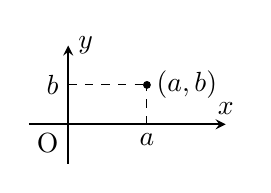
\begin{tikzpicture}
						\draw[->,>=stealth,semithick] (-0.5,0)--(2.0,0)node[above]{$x$};
						\draw[->,>=stealth,semithick] (0,-0.5)--(0,1.0)node[right]{$y$};
						\draw (0,0)node[below left]{O};
						\coordinate (P) at (1,0.5);
						\fill (P) circle (0.05);
						\draw (P) node[right]{$(a,b)$};
						\coordinate (X) at (1,0);
						\coordinate (Y) at (0,0.5);
						\draw[dashed] (X) node[below]{$a$} (X)--(P);
						\draw[dashed] (Y) node[left]{$b$} (Y)--(P);
					\end{tikzpicture}
				\end{tabular}
				\right]
		$左図のように射影のイメージ.
		\begin{tikzcd}
			\mathbb{R} & \mathbb{R}^2 \arrow[l] \arrow[r] & \mathbb{R}
		\end{tikzcd}.

	}
	\begin{quote}
		任意の図式$\langle X,x_1,x_2\rangle$
		\begin{equation}
			\begin{tikzcd}
				A & X \arrow[l,"x_1"'] \arrow[r,"x_2"] & B
			\end{tikzcd}
		\end{equation}
		について以下の図式:
		\begin{equation}
			\begin{tikzcd}
				& X \arrow[ld,"x_1"'] \arrow[d,"u"] \arrow[rd,"x_2"] & \\
				A & P \arrow[l,"p_1"] \arrow[r,"p_2"'] & B
			\end{tikzcd}
		\end{equation}
		を可換にする(すなわち$x_1=p_1u$かつ$x_2=p_2u$)$u:X\to P$が(一意に)存在する.
	\end{quote}
\end{dfn}

直積はco-UMPで定義できる.

\begin{equation}
	\begin{tikzcd}
		&  & (A,B) &  & \\
		& (X,X) \arrow[ur,"{(x_1,x_2)}","\circlearrowright"'] \arrow[r,"{(u,u)}"'] & (P,P) \arrow[u,"{(p_1,p_2)}"'] & \fbox{in $\mathbf{C}\times\mathbf{C}$}\\ [-3.2ex]
		|[alias=X]|\arrow[rrrr,dash,dashed,to=Y] & & & &|[alias=Y]| \\ [-3.2ex]
		& X \arrow[r,dashed,"\exists ! u"] & P & \fbox{in $\mathbf{C}$} \arrow[uu,bend right,"対角関手\Delta\footnotemark"',blue,xshift=2.4em] &
	\end{tikzcd}
\end{equation}
\footnotetext{
	左側と右側の三角形の可換部分を圏の直積を用いてかさねてやる.対角関手$\Delta$は$\left[
			\begin{tabular}{l}
				\begin{tikzcd}
					X \arrow[r,mapsto] \arrow[d,"f"]& (X,X) \arrow[d,"{(f,f)}"] \\
					Y \arrow[r,mapsto] & (Y,Y)
				\end{tikzcd}\end{tabular}
			\right]
	$
	を実現するような関手.
}

\begin{note}
	UMPは2つの部分からなる.
	\begin{itemize}
		\item 存在パート:$\exists u:X\to P$\, s.t.\, $x_1=p_1u$かつ$x_2=p_2u$
		\item 一意性パート:$\forall v:X\to P$\, s.t.\, $p_1 v=x_1$かつ$p_2 v=x_2$,ならば$u=v$
	\end{itemize}

\end{note}

\begin{prop}
	直積は同型を除いて一意的である.
\end{prop}

\begin{proof}
	$\langle P,p_1,p_2\rangle$と$\langle Q,q_1,q_2\rangle$がともに$A$と$B$の直積とする:
	\[
		\begin{tikzcd}
			A & P \arrow[l,"p_1"'] \arrow[r,"p_2"] & B
		\end{tikzcd}
	\]
	\[
		\begin{tikzcd}
			A & Q \arrow[l,"q_1"'] \arrow[r,"q_2"] & B
		\end{tikzcd}
	\]
	$Q$が直積より$i:P\to Q$で$q\circ i=p_1$かつ$q_2\circ i=p_2$となるものが存在.$P$が直積より$j:P\to Q$で$p_1\circ j=q_1$かつ$p_2\circ j=q_2$となるものが存在.

	合成$p_1\circ j\circ i=p_1$,$p_2\circ j\circ i=p_2$.$p_1\circ \mathbbm{1}_P=p_1$,$p_2\circ \mathbbm{1}_P=p_2$より$\blueunderline{j\circ i=\mathbbm{1}_P}{$P\to P$}$($\because$$p$のUMPの一意性)

		同様に$\blueunderline{i\circ j=\mathbbm{1}_Q}{$Q\to Q$}$によって
		\begin{tikzcd}[cramped]
			P \arrow[r,yshift=0.7ex,"i"] & Q \arrow[l,yshift=-0.7ex,"j"]
		\end{tikzcd}
		は同型射($P\cong Q$).
	\begin{equation}
		\begin{tikzcd}[sep=large]
			& P \arrow[ld,"p_1"'] \arrow[d,dashed,"i"] \arrow[rd,"p_2"] \arrow[dd,bend right,blue]& \\
			A & Q \arrow[l,"q_1"'] \arrow[r,"q_2"] \arrow[d,dashed,"j"] & B \\
			& P \arrow[lu,"p_1"] \arrow[ru,"p_2"']
		\end{tikzcd}\footnote{それぞれの部分は可換.}
	\end{equation}
\end{proof}

よって同型な対象の1つを選んで$A\times B$とよぶことにする(集合の場合と同様).

$\mathbf{Set}$でも$P$は集合として一意には決まらない.普通$A\times B=\{(a,b)\mid a\in A,b\in B\}$としているが,$a,b$を取り出す操作(元の情報を取り出すこと\footnote{直積の特徴としてはもとの情報が取り出せるというのがある.例えば行列の積などを考えると演算結果からはもとの行列の情報を取り出すことはできない.})さえできればよいので,たとえば$(a,b)$の代わりに$(a,(a,b))$\footnote{フォン・ノイマンエンコーディング},$((a,b),(a,b))$だって考えることができる.

% 6/7 ここから-----
\startpoint{6/7(第8回)}

$\Set$では射$A\to B$に全射と単射があった.
\begin{itemize}
	\item 単射:$\forall a,a'\in A(f(a)=f(a')\Rightarrow a=a')$
	\item 全射:$\forall b\in B(\exists a\in A(f(a)=b))$
\end{itemize}
これの圏論的な対応物を知る(必ずしも一致するとは限らないことに注意.)

\setcounter{dfn}{0}

\begin{dfn}[エピ射とモノ射]
	$\mathbf{C}$を圏,$f:A\to B$を$\mathbf{C}$の射とする.
	$f$がモノモルフィズム(monomorphism,モノ射,mono)であるとは$\forall g,h:c\rightrightarrows A$\footnote{$c\rightrightarrows A$:parallel pair,平行対.$c$も任意.}について$fg=fh\Rightarrow g=h$\footnote{left cancelable}
	\begin{equation}
		\begin{tikzcd}
			C \arrow[r,yshift=0.7ex,"g"] \arrow[r,yshift=-0.7ex,"h"'] & A \arrow[r,"f"] & B
		\end{tikzcd}
	\end{equation}
	エピモルフィズム(epimorphism,エピ射,epi)であるとは,$\forall i,g:B\rightrightarrows D$\footnote{$D$は任意.}について$if=jf\Rightarrow i=j$\footnote{right cancelable}
	\begin{equation}
		\begin{tikzcd}
			A \arrow[r,"f"] & B \arrow[r,yshift=0.7ex,"g"] \arrow[r,yshift=-0.7ex,"h"'] & D
		\end{tikzcd}
	\end{equation}
	モノ射はよく$A\rightarrowtail B$と書き,エピ射はよく$A\twoheadrightarrow B$と書く\footnote{これらの記号は単射,全射のときによく使われていたらしい.}.
\end{dfn}

\begin{prop}
	集合の間の関数$f:A\to B$がモノモルフィズムであることと$f$が単射であることは同値.
\end{prop}

\begin{proof}
	$f:A\rightarrowtail B$,monoとする.
	$a,a'\in A\textrm{\,\,s.t.\,\,} a\neq a'$\footnote{$A$の要素数が0,1のときは自明に単射になるので2以上を考える.}
	$\{x\}$を1対象集合\footnote{singleton set(one-object set)}とする.
	$\overline{a},\overline{a'}:\{x\}\to A$
	を$\overline{a}(x)=a,\overline{a'}(x)=a'$で定義する.
	モノ射の条件の対偶\footnote{$\overline{a}\neq\overline{a'}\Rightarrow f\overline{a}\neq f\overline{a'}$.関数の合成は積のように書いている.}と$a\neq a'$より$f\overline{a}\neq f\overline{a'}$.
	よって$f(a)=(f\overline{a})(x)\neq(f\overline{a'})(x)=f(a')$
	ゆえに$f$は単射\footnote{$a\neq a'\Rightarrow f(a)\neq f(a')$が示せた.}である.

	逆に$f$は単射とする.$g,h:C\to A$が$g\neq h$である関数とする.このときある$c\in C$について$g(c)\neq h(c)$(外延性).$f$が単射より$f(g(c))\neq f(h(c))$.ゆえに$fg\neq fh$なのでモノ射の条件の対偶が成り立つ.
\end{proof}

よく現れる圏では単射的準同型\footnote{集合+構造という数学的対象と,その構造を保存する関数をもつ圏はこうなることが多い.$\Mon,\mathbf{Grp},\mathbf{Ring}$など.}はモノ射になることが多い.

\begin{ex}[$\Mon$]
	モノイド準同型$h:M\to N$\footnote{\fbox{in $\Mon$}.$M,N$はモノイド.}がモノ射であれば台関数$|h|:|M|\to|N|$\footnote{\fbox{in $\Set$}.}もモノ射,すなわち単射である.逆も成り立つ.
\end{ex}

\begin{proof}
	$h$をモノ射とし,$1=\{*\}$を1対象集合(1点集合),$x,y:1\to|M|$であって$x(*)\neq y(*)$であるものとする($|M|$の"要素"\footnote{
		\begin{tikzcd}
			\{*\} \arrow[d,phantom,"\rotatebox{90}{$\in$}"] \arrow[r,"\hat x"] & S \arrow[d,phantom,"\rotatebox{90}{$\in$}"] \\[-2ex]
			* \arrow[r,mapsto] & x
		\end{tikzcd}
		実際には$x$が要素だが,写像$\hat x$を指定することと要素$x$を指定することは等価なので,$\hat x$を要素とみなしてもよいだろう,ということ.
	}).
	自由モノイド$M(1)$のUMPより\footnote{
		\begin{tikzcd}
			& M(1) \arrow[r,dashed,"\exists !\overline{x}"] & M & \fbox{in $\Mon$} & \\ [-3.2ex]
			|[alias=X]|\arrow[rrrr,dash,dashed,to=Y] & & & &|[alias=Y]| \\ [-3.2ex]
			& {|M(1)|}\arrow[r,"|\overline{x}|"] & {|M|} & \fbox{in $\Set$} & \\
			& 1 \arrow[u,"\quad\circlearrowright"'] \arrow[ru,"\forall x"']
		\end{tikzcd}
		$\forall x$について$\exists ! \overline{x}$が対応.$x$に対して異なる$y$をとれば$\overline{y}$も異なる.
	},異なる準同型$\overline{x},\overline{y}:M(1)\to M$が存在し,$h$がモノ射であることより,以下の合成は異なる.
	\[
		h\circ \overline{x},h\circ \overline{y}:M(1)\to M\to N
	\]
	よって対応する$|N|$の"要素"も異なる.
	\[
		\begin{tikzcd}
			M(1) \arrow[d,blue,"{|\cdot|}"',bend right,xshift=-1.6em] \arrow[r,yshift=0.7ex,"\overline{x}"] \arrow[r,yshift=-0.7ex,"\overline{y}"'] & M \arrow[r,"h"] & N \\
			1 \arrow[r,yshift=0.7ex,"x"] \arrow[r,yshift=-0.7ex,"y"'] & {|M|} \arrow[r,"{|h|}"] & {|N|}
		\end{tikzcd}
	\]

	逆に$|h|:|M|\to |N|$がモノ射
	$f,g:X\to M$が異なる準同型のとき($f\neq g$),$|f|,|g|:|X|\to|M|$は異なる関数であり,$|h|$がモノ射なので$|h|\circ|f|,|h|\circ g:|X|\to |M|\to |N|$も異なる関数である.
	よって$|h\circ f|=|h|\circ |f|\neq |h|\circ |g|=|h\circ g|$なので$h\circ f\neq h\circ g$.よって$h$はモノ射.
\end{proof}

双対的に$\Set$ではエピ射は全射である.しかしよく現れる圏ではエピ射は全射的準同型でないことが多い.

\setcounter{dfn}{4}

\begin{ex}
	$\Mon$においてモノ射$\mathbf{N}\rightarrowtail \mathbf{Z}$を考える.ただし$\mathbf{N}=(N,+,0)$,$\mathbf{Z}=(Z,+,0)$.このモノ射は台関数として包含写像$N\hookrightarrow Z$をもつ($\Set$のエピ射でない)がこれは$\Mon$においてエピ射である.
\end{ex}

\begin{proof}
	モノイド準同型$f,g:(\mathbf{Z},+,0)\to(M,*,u)$で$f|_N=g|_N$ならば$f=g$をみたすものとする.
	\[
		f(-n)=f((-1)_1+(-1)_2+\cdots +(-1)_n)=f(-1)_1*f(-1)_2*\cdots *f(-1)_n
	\]
	であり$g$も同様であることにして注意すると
	\[
		\begin{split}
			f(-1)
			&=f(-1)*u \\
			&=f(-1)*g(0) \\
			&=f(-1)*g(1-1) \\
			&=f(-1)*g(1+(-1)) \\
			&=f(-1)*g(1)*g(-1) \\
			&=f(-1)*f(1)*g(-1) \\
			&=f(-1+1)*g(-1) \\
			&=f(0)*g(-1) \\
			&=u*g(-1) \\
			&=g(-1)
		\end{split}
	\]
\end{proof}

\begin{prop}
	同型射は\footnote{$p$が同型射$\defLeftrightarrow \exists q\,\,\textrm{s.t.}\,\, q\circ p=1_X,p\circ q=1_Y$}モノ射かつエピ射である.
\end{prop}

\begin{proof}
	\begin{equation}
		\begin{tikzcd}
			A \arrow[r,yshift=0.7ex,"x"] \arrow[r,yshift=-0.7ex,"y"'] & B \arrow[r,"m"] \arrow[rd,"\mathbbm{1}"] & C \arrow[d,"e"] & \\
			& & B \arrow[r,yshift=0.7ex,"u"] \arrow[r,yshift=-0.7ex,"v"'] & D
		\end{tikzcd}
	\end{equation}
	$m$が同型射で逆射$e$をもつとき,$mx=my$ならば$x=emx=emy=y$.よって$m$はモノ射.
	同様に$e$は同型射であり逆射$m$をもつとき$ue=ve$ならば$u=uem=vem=v$.よって$r$はエピ射
\end{proof}

\subsubsection{セクションとレトラクション}

より一般的に$f:A\to B$が左逆射$g:B\to A,gf=\mathbbm{1}_A$をもつとき,$f$はモノ射で$g$はエピ射であることも同様の議論で示せる.\footnote{同型射の条件のうち片方だけしか持たない場合はどうなるかというお話.
}

\begin{dfn}[分裂モノ射(split mono),分裂エピ射(split epi),セクション,レトラクション]
	分裂モノ射は左逆射をもつ射である.
	分裂エピ射は右逆射をもつ射である.
	射$e:X\to A$と$s:A\to X$が$es=\mathbbm{1}_A$をみたすとき$s$は$e$のセクションもしくはsplitingと呼ばれ,$e$は$s$のレトラクションと呼ばれる.対象$A$は$X$のレトラクトと呼ばれる.
	\footnote{
		セクションのイメージ.
		\begin{center}
			\begin{tikzpicture}
				\draw (-1.5,-1) -- (1.5,-1) -- (1.5,1) -- (-1.5,1) -- (-1.5,-1);
				\draw[domain=-1.5:1.5] plot(\x, {1.5*log10(\x+2+2*sin(\x*\x))*cos(\x)+3*sin(4*\x)-2*sin(7*\x)+0.05*\x*\x*\x-0.1});
				\draw (-0.5,1)--(-0.5,-1);
				\draw (1,1)--(1,-1);
				\draw [dashed](-0.5,-1)--(-0.5,-2);
				\draw [dashed](1,-1)--(1,-2);
				\fill (-0.5,-2) circle [radius=1pt];
				\fill (1,-2) circle [radius=1pt];
				\draw (-1.5,-2)--(1.5,-2);

				\node (X) at (-2,0) {$X$};
				\node (A) at (-2,-2) {$A$};
				\draw [->,transform canvas={xshift=2pt}](X) -- node [midway, right]{$\scriptstyle e$} (A);
				\draw [->,transform canvas={xshift=-2pt}](A) -- node [midway, left]{$\scriptstyle s$} (X);

				\draw [<-] (1.53,0.83) -- (1.8,0.83) node [right]{section(横断のイメージ)};
			\end{tikzpicture}
		\end{center}
		レトラクションのイメージ.
		$e:X\to A$に対して$\tilde e:X\to X$を$\tilde e(x)\defeq e(x)$で定める.このとき$a\in A$は$\tilde e(a)=a\in A$となり$A$は不変な部分となっている.
		\begin{center}
			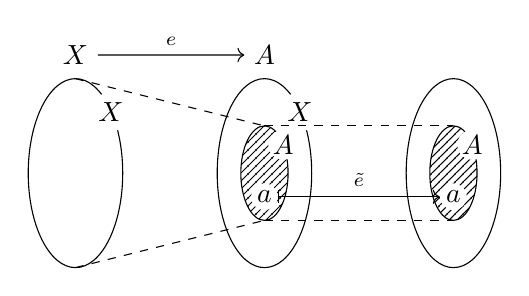
\begin{tikzpicture}[scale=0.6]
				\node (A) at (0,2.5) {$X$};
				\node (B) at (4,2.5) {$A$};

				\draw [->] (A) -- node [midway, above]{$\scriptstyle e$} (B);

				\draw (0,0) ellipse [x radius=1,y radius=2];
				\node [fill=white,circle,inner sep=1pt] (X0) at (0.75,1.3) {$X$};

				\draw [dashed] (0,2) -- (4,1);
				\draw [dashed] (0,-2) -- (4,-1);

				\draw (4,0) ellipse [x radius=1,y radius=2];
				\filldraw [pattern=south west lines] (4,0) ellipse [x radius=0.5,y radius=1];
				\node [fill=white,circle,inner sep=1pt] (X1) at (4.75,1.3) {$X$};
				\node [fill=white,circle,inner sep=0.25pt] (A1) at (4.4,0.6) {$A$};

				\node [fill=white,circle,inner sep=1pt] (a) at (4,-0.5) {$a$};

				\draw [dashed] (4,1) -- (8,1);
				\draw [dashed] (4,-1) -- (8,-1);

				\draw (8,0) ellipse [x radius=1,y radius=2];
				\filldraw [pattern=south west lines] (8,0) ellipse [x radius=0.5,y radius=1];
				\node [fill=white,circle,inner sep=0.25pt] (A1) at (8.4,0.6) {$A$};

				\node [fill=white,circle,inner sep=1pt] (ea) at (8,-0.5) {$a$};

				\draw [|->] (a) -- node [midway, above]{$\scriptstyle \tilde e$} (ea);

			\end{tikzpicture}
		\end{center}
	}
\end{dfn}

\subsection{Generalized Element}

任意の集合$X$について
\begin{equation}
	\begin{tikzcd}[row sep=0.2ex]
		X \arrow[r,phantom,"\cong"] \arrow[d,phantom,"\rotatebox{90}{$\in$}"]& \Hom_{\Set}(1,X) \arrow[d,phantom,"\rotatebox{90}{$\in$}"] & &\\
		x \arrow[r,mapsto] & \overline{x}\footnotemark
	\end{tikzcd}
\end{equation}
\footnotetext{
	\begin{tikzcd}[row sep=0.2ex]
		1 \arrow[r,"\overline{x}"] \arrow[d,phantom,"\rotatebox{90}{$\in$}"] & X \arrow[d,phantom,"\rotatebox{90}{$\in$}"]\\
		* \arrow[r,mapsto] & x
	\end{tikzcd}\\
	$\Hom_{\Set}(1,X)$は$1$から$X$への圏$\Set$における集合$1$から集合$X$へのすべての関数を集めた集合である.
}
$1=\{*\}$は$\Set$の終対象.すなわち集合$X$の要素$x$は$\overline{x}$と同型により同一視できる.
これを一般化して終対象$1$をもつ任意の圏において射$1\to A$は$A$のglobal element,point,constantと呼ばれる.
$\Set,\Pos,\mathbf{Top}$では
$f,g:A\to B$について任意のpoint\,$a:1\to A$との合成が$fa=ga$ならば$f=g$.よって射はドメインのpointで決まる.

しかし常にこれが成り立つわけではない.より一般的に任意の圏においてgeneralized elementという概念を導入しよう.
対象$A$のgeneralized element(一般化要素)とは射$X\to A$である($X$は任意のtest object)\footnote{この$X$には終対象であるといった条件はなく,任意である.test objectなどという.}.

% 6/14 ここから -----------

\startpoint{6/14(第9回)}

\subsection{積をもつ圏}

$\mathbf{C}$を,すべての対象の組$(A,A')$について積(図式)
\begin{equation}
	\begin{tikzcd}[row sep=0.4ex]
		A & P \arrow[l,"p_1"'] \arrow[r,"p_2"] \arrow[d,phantom,"\rotatebox{90}{$=$}"]& A' \\
		& A\times A' &
	\end{tikzcd}
\end{equation}
をもつ圏とする.\footnote{圏の直積はペアで定義した$\Rightarrow\mathbf{CAT}$二項積になっている}

\begin{equation}
	\begin{tikzcd}[row sep=large,column sep=large]
		|[alias=A]| A \arrow[d,"f"'] & A\times A' \arrow[l,"p_1"'] \arrow[r,"p_2"]
		\arrow[ld,blue,rounded corners,to path={(\tikztostart.south west)--(A.south east)--(\tikztotarget.north east)}]
		\arrow[rd,blue,rounded corners,to path={(\tikztostart.south east)--(Ad.south west)--(\tikztotarget.north west)}]
		\arrow[d,red,dashed,"f\times f'"] & |[alias=Ad]| A' \arrow[d,"f'"] \\
		B & B\times B' \arrow[l,"q_1"] \arrow[r,"q_2"'] & B'
	\end{tikzcd}
\end{equation}
このとき$f\times f'\defLeftrightarrow \langle f\circ p_1,f'\circ p_2\rangle$とおくとこの射が一意的に存在する.すると$\times:\mathbf{C}\times\mathbf{C}\to \mathbf{C}$($(f,f')\mapsto f\times f'$)という関手が得られる(関手性はUMPから容易にチェックできる.).

そのような圏は(すべての)(2項)積をもつという.

同様なUMPにより3項の積$A_1\times A_2\times A_3$も定義できる\footnote{
	3項の積の図式は
	$\left[
			\begin{tabular}{l}
				\begin{tikzcd}
					& A_1\times A_2\times A_3 \arrow[dl,"p_1"'] \arrow[d,"p_2"'] \arrow[dr,"p_3"]\\
					A_1 & A_2 & A_3
				\end{tikzcd}
			\end{tabular}
			\right]$
}.対象$A_1\times A_2\times A_3$と3つの射$P_i:A_1\times A_2\times A_3\to A_i$で次のUMP\footnote{2項の積のときは$\mathbf{C}$と$\mathbf{C}\times\mathbf{C}$との間のUMPを考えたが,3項のときは$\mathbf{C}$と$\mathbf{C}\times \mathbf{C}\times \mathbf{C}$とのUMPを考える.}をみたす:
\begin{quote}
	任意の$X,X_i:X\to A_i$($i=1,2,3$)について$u\circ p_i=x_i$をみたす$u$が一意的に存在する\footnote{以下で$X,x_1,x_2,x_3$は任意.}
	\[
		\begin{tikzcd}[row sep=huge]
			& A_1\times A_2\times A_3 \arrow[dl,"p_1"'] \arrow[d,"p_2"',near start] \arrow[dr,"p_3",near end]& X \arrow[l,dashed,"\exists ! u"'] \arrow[lld,"x_1",near end] \arrow[ld,"x_2",near end] \arrow[d,"x_3"] \\
			A_1 & A_2 & A_3
		\end{tikzcd}
	\]
\end{quote}
ものが定義できる(この時点で3項の積の存在は言っていない).同様に任意の自然数$n$項の積が定義できる.

一方で任意の対象$A,B,C$について2項積を2回とることにより$(A\times B)\times C$は必ず存在する.これのUMPと3項積のUMPにより(もしくは2項積のUMPを複数回用いることで)
\[
	A\times B\times C\cong (A\times B)\times C
\]
が示せる(up to iso).よって,例えば
\[
	A\times B\times C=(A\times B)\times C
\]
とおくことができる(on the nose).すると,3項積のUMPにより
\[
	(A\times B)	\times C\cong A\times (B\times C)
\]
が示せる\footnote{
	in $\Set$では$A\times B=\{(a,b)\mid a\in A\land b\in B\}$として$((a,b),c)\in(A\times B)\times C, (a,(b,c))\in A\times (B\times C)$これら2つは通常の数学では同一視していることが多い.
}.よって$\times$は結合律を同型を除いて満たすことがわかる($n\geq 2$\footnote{ここまでは暗に$n\geq 2$で考えていた.}).さらに$n=0$の場合に整合的に拡張することを考える.すなわち,ある対象1が存在して,任意の対象$X$について一意的な射
\[
	!:X\to 1
\]
が存在するという条件が相当する\footnote{\begin{tikzcd} A & \arrow[l,dashed,"\exists ! u"'] \forall X \end{tikzcd}}.これは$\mathbf{C}$に終対象1つが存在するという主張に他ならない.
$n=1$の場合はなにもしないことに相当する(正確には同型のずれは許容する).よって任意の有限集合$I$(すなわち(有限の)離散圏\footnote{
	オブジェクトごとに恒等射しかない圏のこと.例えば
	$\left[
			\begin{tabular}{l}
				\begin{tikzcd}
					\cdot \arrow[out=30,in=330,loop] & \cdot \arrow[out=30,in=330,loop] & \cdot \arrow[out=30,in=330,loop]
				\end{tikzcd}
			\end{tabular}
			\right]$
	という圏.
})について対象の族$\{C_i\}_{i\in I}$を考えると,$I$項の積を考えることができる\footnote{
	後に任意の小圏に拡張することを念頭に置いている.
}.

\setcounter{dfn}{18}

\begin{dfn}
	圏$\mathbf{C}$がすべての有限積をもつとは,終対象とすべての2項積をもつ(すなわち,すべての有限個数の積をもつ)ことである.圏$\mathbf{C}$がすべての(スモールな)積をもつとは,対象の任意の集合が積をもつことである\footnote{後半は有限という条件を外したもの.}.
\end{dfn}

(注意:集合,すなわち離散圏の場合だけでなく任意の小圏に一般化した議論を後に行う.)

\subsection{Hom集合}

本節では圏はすべて局所小とする.圏$\mathbf{C}$の任意の対象$A,B$について$A$から$B$への射全体のなす集合を$\Hom(A,B)=\{f\in\mathbb{C}|f:A\to B\}$と書いたことを思い出そう.この射の集合をHom集合と呼ぶ.

(板書ここまで.以下教科書と板書のメモを元に作成)

$g:B\to B'\in\mathbf{C}$が誘導する(induce)関数を定義する.
\[
	\begin{split}
		\Hom(A,g):\Hom(A,B)\to \Hom(A,B') \\
		(f:A\to B)\mapsto (g\circ f:A\to B\to B')
	\end{split}
\]
$Hom(A,g)=g\circ f$.しばしば$\Hom(A,g)$を$g_*$と書く\footnote{圏論がメインでない文献ではよくある}.
\[
	\begin{tikzcd}[column sep=12em,row sep=huge,remember picture]
		& B \arrow[dd,"g"] \\
		A \arrow[ru,""{name=UAB}] \arrow[ru,bend left=10] \arrow[ru,bend right=10,"f"{name=U, below},near end] \arrow[rd,""{name=DABd}] \arrow[rd,bend left=10,"g\circ f"{name=D},near end] \arrow[rd,bend right=10]\\
		& B'
		\arrow[mapsto,from=U,to=D]
	\end{tikzcd}
	\begin{tikzpicture}[overlay,remember picture]
		\draw[dashed] (UAB) circle (0.6);
		\draw[dashed] (DABd) circle (0.6);
		\node[above=3ex,left=1.5em] (HomAB) at (UAB) {$\scriptstyle \Hom(A,B)$};
		\node[below=3ex,left=1.5em] (HomABd) at (DABd) {$\scriptstyle \Hom(A,B')$};
		\draw[->] (HomAB) -- node[right] {$\scriptstyle \Hom(A,g)=g_*$} (HomABd);
	\end{tikzpicture}
\]
$g\in\mathbf{C}$を動かした時に射が定まる各オブジェクトごとに集合が決まり,各射ごとに写像が定まるので関手が定まると考えられる.
\[
	\Hom(A,-):\mathbf{C}\to\Set
\]
これを$A$の(covariant) replesentable functor\footnote{
	representableとは$A$からの射ですべて情報が確定する(関手が表現できる)という意味でrepresentableと言う。
	あまり気にしなくて良いがcovariant functor(共変関手)は射の向きが同じになるもの.つまり
	\[
		\begin{tikzcd}
			\Hom(A,-): &[-3em] \mathbf{C} \arrow[r] & \Set \\[-2ex]
			& B \arrow[d,"g"] & \Hom(A,B) \arrow[d,"g_*"]\\
			& B' & \Hom(A,B')
		\end{tikzcd}
	\]
	となるもの.それに対して
	\[
		\begin{tikzcd}
			F: &[-3em] \mathbf{C} \arrow[r] & \mathbf{D} \\[-2ex]
			& A \arrow[d,"f"] & F(A) \\
			& A' & F(A') \arrow[u,"F(f)"]
		\end{tikzcd}
	\]
	ではなく(これは我々の考える関手の定義を満たさない),
	\[
		\begin{tikzcd}
			F: &[-3em] \mathbf{C}^{\textrm{op}} \arrow[r] & \mathbf{D} \\[-2ex]
			& A  & F(A) \\
			& A' \arrow[u,"f"] & F(A') \arrow[u,"F(f)"]
		\end{tikzcd}
	\]
	を考えれば関手になり,これをcovariant functor(反変関手)という.
}という.これが関手性を満たすことも確認できる(教科書p.44参照).

ここで積の定義をホムセットで書き直してみよう.対象$P$と射$p_1:P\to A$,$p_2:P\to B$からなる組$(P,p_1,p_2)$を考える.いま
\[
	(p_1,p_2)\in\Hom(P,A)\times \Hom(P,B)
\]
(ここの$\times$は集合の直積)をとってきたとしよう.任意の射$x:X\to P$をとり,$x_1=p_1\circ c:X\to A$と$x_2=p_2\circ c:X\to A$を定める.

このように定めると以下のような関数が定まる.
\[
	\begin{tikzcd}
		\vartheta_X=(\Hom(X,p_1),\Hom(X,p_2)): &[-4ex] \Hom(X,P) \arrow[r] \arrow[d,phantom,"\rotatebox{90}{$\in$}"] & \Hom(X,A)\times \Hom(X,B) \arrow[d,phantom,"\rotatebox{90}{$\in$}"] \\[-2ex]
		& x \arrow[r,mapsto] & (x_1,x_2)
	\end{tikzcd}
\]
つまり
\[
	\vartheta_X(x)=(x_1,x_2)
\]
で定義される.

\begin{prop}
	以下の図式
	\[
		\begin{tikzcd} A & P \arrow[l,"p_1"] \arrow[r,"p_2"] & B\end{tikzcd}
	\]
	が$A$と$B$の積であるための必要十分条件は,任意の対象$X$と$\vartheta_X(x)=(x_1,x_2)$で定義されているcanonical function $\vartheta_X$が同型であることである:
	\[
		\vartheta_X:\Hom(X,P)\cong \Hom(X,A)\times\Hom(X,B)
	\]
\end{prop}

\begin{proof}
	省略(教科書参照)
\end{proof}

\begin{dfn}
	$\mathbf{C},\mathbf{D}$を2項積の圏とする.関手$F:\mathbf{C}\to \mathbf{D}$が2項積を保存するというのは
	\[
		\begin{tikzcd}
			A & A\times B \arrow[l,"p_1"] \arrow[r,"p_2"] & B & \fbox{in $\mathbf{C}$}
		\end{tikzcd}
	\]
	を$F$でうつしたとき
	\[
		\begin{tikzcd}
			F(A) & F(A\times B) \arrow[l,"F(p_1)"] \arrow[r,"F(p_2)"] & F(B) & \fbox{in $\mathbf{D}$}
		\end{tikzcd}
	\]
	となっていることである.

	これは一般に
	\[
		\begin{tikzcd}
			F(A) & F(A)\times F(B) \arrow[l,"q_1"'] \arrow[r,"q_2"] & F(B)
		\end{tikzcd}
	\]
	とは必ずしも一致しないが,
	\[
		F(A\times B)\cong F(A)\times F(B)
	\]
	が"カノニカル"に同型\footnote{"canonically"や"カノニカル"は正確な用語ではないのであまり気にしなくてよい.}であればよい,つまり
	\[
		\langle F(p_1),F(p_2) \rangle :F(A\times B)\to F(A)\times F(B)\quad \fbox{in $\mathbf{D}$}
	\]
	という射$\langle F(p_1),F(p_2) \rangle$を構成できるという意味で定められた同型である.
\end{dfn}

% 6/21 ここから ----------
\startpoint{6/21(第10回)}

\section{双対性}

教科書参照.\url{http://www.andrew.cmu.edu/course/80-413-713/notes/chap03.pdf}

\end{document}
